\PassOptionsToPackage{dvipsnames,svgnames,x11names}{xcolor}
\documentclass[runningheads]{llncs}
\usepackage[T1]{fontenc}
\usepackage{hyperref}
\usepackage{graphicx}
\usepackage{multirow}
\usepackage{amsmath,amssymb,amsfonts}
\usepackage{mathrsfs}
\usepackage{appendix}
\usepackage{xcolor}
\usepackage{textcomp}
\usepackage{manyfoot}
\usepackage{booktabs}
\usepackage{algorithm}
\usepackage{algorithmicx}
\usepackage{tabularx}
\usepackage{algpseudocode}
\usepackage{listings}
\usepackage{csquotes}
\usepackage{placeins}
\usepackage{float}
\usepackage{caption}
\usepackage{tikz}
\usetikzlibrary{positioning, arrows.meta, shapes.geometric, fit, backgrounds}


\begin{document}

\title{Predictive Analysis of Autism Spectrum Disorder Traits: Integrating Quantum Machine Learning and Exploratory Data Insights}
\author{Subhra Kolay\inst{1}\orcidID{0009-0002-4625-5941} \and
Srijan Samaddar\inst{2}\orcidID{0009-0001-5799-016X} \and
Ayushman Bhattacharya\inst{1}\orcidID{0009-0006-5960-6308} \and
Bidisha Bhabani\inst{1}\orcidID{0000-0003-4261-1849}\and
Tanaya Das\inst{1}\orcidID{0000-0001-9196-973} \and
Sohrab Siddique\inst{1}\orcidID{0009-0000-5743-6882} \and
Ilora Maity\inst{3}\orcidID{0000-0002-8042-4123}}

\institute{Department of Computer Science and Engineering, JIS University,\
Kolkata, West Bengal, India\\
\email{subhrokolay2@gmail.com, bhattacharyaa599@gmail.com,\\
        bidisha035810@gmail.com, tanaya.das@jisuniversity.ac.in,\\
        sksohrabsiddique123@gmail.com}
\and
Department of Information Technology, Netaji Subhash Engineering College, West Bengal, India\\
\email{srijansamaddar04@gmail.com}
\and
Interdisciplinary Centre for Security, Reliability and Trust (SnT),\\
University of Luxembourg, Luxembourg City, Luxembourg\\
\email{ilora.maity@uni.lu}}

\maketitle
\raggedbottom
\abstract{
This research presents a head-to-head comparison of Classical Machine Learning (CML) and Quantum Machine Learning (QML) for binary classification, using a clinically validated ASD screening dataset of 3{,}744 instances as a shared benchmark to evaluate whether near-term quantum approaches can match established classical methods on a real-world diagnostic task. Seven classical supervised models---including Logistic Regression, SVM, Random Forest, and Histogram Gradient Boosting Classifier (HGBC)---were evaluated alongside three quantum models: Variational Quantum Classifier (VQC), Quantum Support Vector Machine (QSVM), and Quantum Naive Bayes (QNB), all operating on the same PCA-reduced feature space to ensure a fair comparison. Among all models, HGBC achieved the highest performance with 97.86\% accuracy, 98.48\% precision, 97.50\% recall, and a 97.90\% F1-score. Among quantum models, QSVM achieved the best accuracy at 77.30\%. Exploratory Data Analysis on demographic attributes revealed higher ASD trait prevalence in children (60.57\%) and males, along with patterns related to ethnicity and family history. The results demonstrate that classical ensemble methods remain superior for this binary classification task under current quantum hardware constraints, while QML approaches offer a promising direction for future work on more complex, high-dimensional feature spaces.
} \\

\keywords{Autism Spectrum Disorder (ASD), Quantum Machine Learning, Classification Algorithms, HGBC, QSVM, Variational Quantum Classifier}


\section{Introduction}\label{sec1}
Quantum Machine Learning (QML) has emerged as a potential alternative to classical supervised methods, with theoretical work suggesting that certain quantum models can exploit high-dimensional Hilbert spaces to capture non-linear feature relationships more efficiently than their classical counterparts \cite{saranya2025}. However, a critical open question remains: \emph{can near-term quantum classifiers match or exceed the performance of well-tuned classical models on real-world binary classification tasks?}

This paper addresses that question through a controlled, head-to-head comparison of Classical Machine Learning (CML) and QML on a common benchmark. We adopt a clinically validated Autism Spectrum Disorder (ASD) screening dataset \cite{asddataset} comprising 3{,}744 instances and 17 features as our testbed---not to advance ASD diagnosis per se, but because the dataset offers a well-structured, near-balanced binary classification problem with both linear and non-linear feature interactions, making it an ideal proving ground for comparing the two paradigms.

Seven classical supervised models---including Logistic Regression, SVM, Random Forest, and Histogram Gradient Boosting Classifier (HGBC)---are evaluated alongside three quantum models: a Variational Quantum Classifier (VQC), a Quantum Support Vector Machine (QSVM), and a Quantum Naive Bayes (QNB) hybrid. All models are trained and tested on the same data partitions, and quantum models operate on the same PCA-reduced feature space to ensure a fair comparison. The quantum circuits are implemented using PennyLane and Qiskit simulation frameworks.

The key contributions of this research are:
\begin{itemize}
\item A rigorous CML vs QML benchmark on a shared dataset with identical preprocessing, train-test splits, and evaluation metrics, enabling direct performance comparison.
\item Implementation and detailed circuit-level description of three distinct quantum classifiers---VQC (trainable ansatz), QSVM (quantum kernel), and QNB (parameterless feature map)---each representing a different QML paradigm.
\item Justification of the 4-qubit, 4-PCA-component design and analysis of how quantum angle encoding transforms classical features into Hilbert space.
\item Exploratory Data Analysis on demographic attributes to contextualise the dataset and characterise the study population.
\end{itemize}

\section{Related Works}\label{sec2}
The application of Machine Learning to binary classification on tabular datasets is well established, and the ASD screening domain provides a representative case study. Prior work in this space can be grouped into classical and quantum approaches, both of which inform our comparative methodology.

Within the classical Machine Learning (CML) domain, supervised models such as Random Forest (RF) and Support Vector Machines (SVM) have consistently achieved strong results on questionnaire-based ASD datasets \cite{vakadkar2021}. These algorithms are attractive for their robustness to noisy features and ability to model non-linear decision boundaries. However, when scaled to large sample sizes or high-dimensional feature spaces, many classical models exhibit computational complexities on the order of $O(N^2)$ or $O(N^3)$, which can limit their applicability to truly large-scale problems.

On the quantum side, recent theoretical work has suggested that certain QML models can achieve runtime scaling as $O(\text{poly}(\log N) \cdot \text{poly}(D))$, where $D$ denotes the feature dimension, offering a polynomial improvement over many classical counterparts \cite{saranya2025}. Quantum kernel methods \cite{havlivcek2019} and variational classifiers \cite{schuld2020} have been proposed as near-term approaches that leverage quantum feature spaces for classification, though their practical advantage on moderately sized datasets remains an open question.

Despite these advances, several methodological gaps persist in existing CML--QML comparisons. Many prior studies rely on relatively small or imbalanced datasets, which can bias classifiers toward majority classes and inflate performance metrics \cite{lee2020}. Others evaluate classical and quantum models under different preprocessing pipelines or train-test splits, making direct comparison unreliable.

Our work addresses these gaps by benchmarking CML and QML models on a shared, near-balanced dataset with identical preprocessing, stratified splits, and evaluation metrics. This controlled setup allows us to rigorously assess where quantum models stand relative to classical methods on a real-world binary classification task \cite{vakadkar2021,saranya2025,lee2020,nogay2020}.

% ---------------------------------------------------------------
% SECTION 3: METHODOLOGY
% Fix 1: Removed \FloatBarrier before the workflow figure and
%         changed [H] to [!htbp] so LaTeX can place the figure
%         naturally at the top of the page, eliminating the gap
%         that appeared between the section heading and the figure.
% ---------------------------------------------------------------
\section{Methodology}\label{sec3}

\begin{figure}[!htbp]
    \centering
    \definecolor{boxblue}{RGB}{70,130,180}
    \definecolor{boxbluefill}{RGB}{220,235,245}
    \definecolor{boxgreen}{RGB}{60,140,60}
    \definecolor{boxgreenfill}{RGB}{220,240,220}
    \definecolor{boxorange}{RGB}{210,140,50}
    \definecolor{boxorangefill}{RGB}{250,235,210}
    \definecolor{boxgrayborder}{RGB}{150,150,150}
    \definecolor{boxgrayfill}{RGB}{230,230,230}
    \definecolor{arrgray}{RGB}{130,130,130}
    \definecolor{dashgray}{RGB}{170,170,170}
    \definecolor{boxred}{RGB}{234,126,126}
    \resizebox{\linewidth}{!}{%
    \begin{tikzpicture}[
        node distance=0.55cm and 1.8cm,
        >={Stealth[length=3pt]},
        bluebox/.style={rectangle, rounded corners=2pt, draw=boxblue, fill=boxbluefill,
                     text width=2.6cm, minimum height=0.7cm, align=center, font=\small},
        greenbox/.style={rectangle, rounded corners=2pt, draw=boxgreen, fill=boxgreenfill,
                     text width=2.6cm, minimum height=0.7cm, align=center, font=\small},
        orangebox/.style={rectangle, rounded corners=2pt, draw=boxorange, fill=boxorangefill,
                     text width=2.6cm, minimum height=0.7cm, align=center, font=\small},
        redbox/.style={rectangle, rounded corners=2pt, draw=red, fill=boxred, text=white,
                     text width=2.6cm, minimum height=0.7cm, align=center, font=\small},
        graybox/.style={rectangle, rounded corners=2pt, draw=boxgrayborder, fill=boxgrayfill,
                     text width=2.6cm, minimum height=0.7cm, align=center, font=\small},
        colhead/.style={font=\bfseries\small, align=center},
        dashedbox/.style={draw=dashgray, dashed, rounded corners=4pt, inner sep=8pt},
        arr/.style={->, thick, arrgray},
        darr/.style={->, dashed, thick, dashgray},
    ]

    % ── Dataset node ──
    \node[bluebox, text width=2.2cm, minimum height=0.65cm,
          font=\small\bfseries] (dataset) {Dataset};

    % ════════════════  CML column  ════════════════
    \node[colhead, below left=1.2cm and 3.6cm of dataset] (cml-title)
          {\textsf{CML}\\[-1pt]{\scriptsize(Classical ML)}};
    \node[bluebox, below=0.35cm of cml-title]  (cml-raw)  {Raw Features $\mathbb{R}^{n}$};
    \node[greenbox, below=0.45cm of cml-raw]  (cml-model){Classical Model};

    % ════════════════  PCA-CML column  ════════════════
    \node[colhead, below=1.2cm of dataset] (pca-title)
          {\textsf{PCA--CML}\\[-1pt]{\scriptsize(PCA + Classical ML)}};
    \node[bluebox, below=0.35cm of pca-title]  (pca-raw)  {Raw Features $\mathbb{R}^{n}$};
    \node[bluebox, below=0.45cm of pca-raw]   (pca-red)  {PCA Reduction};
    \node[greenbox, below=0.45cm of pca-red]   (pca-model){Classical Model};

    % ════════════════  QML column  ════════════════
    \node[colhead, below right=1.2cm and 3.6cm of dataset] (qml-title)
          {\textsf{QML}\\[-1pt]{\scriptsize(Quantum ML)}};
    \node[bluebox, below=0.35cm of qml-title]  (qml-raw)  {Raw Features $\mathbb{R}^{n}$};
    \node[bluebox, below=0.45cm of qml-raw]   (qml-red)  {PCA Reduction};
    \node[orangebox, below=0.45cm of qml-red]   (qml-enc)  {Angle Encoding};
    \node[redbox, below=0.45cm of qml-enc]   (qml-circ) {Quantum Circuit};
    \node[graybox, below=0.45cm of qml-circ]  (qml-meas) {Measurement};

    % ── Dashed bounding boxes ──
    \begin{scope}[on background layer]
      \node[dashedbox, fit=(cml-title)(cml-raw)(cml-model)] (cml-box) {};
      \node[dashedbox, fit=(pca-title)(pca-raw)(pca-model)] (pca-box) {};
      \node[dashedbox, fit=(qml-title)(qml-raw)(qml-meas)]  (qml-box) {};
    \end{scope}

    % ── Arrows inside columns ──
    \draw[arr] (cml-raw)  -- (cml-model);

    \draw[arr] (pca-raw)  -- (pca-red);
    \draw[arr] (pca-red)  -- (pca-model);

    \draw[arr] (qml-raw)  -- (qml-red);
    \draw[arr] (qml-red)  -- (qml-enc);
    \draw[arr] (qml-enc)  -- (qml-circ);
    \draw[arr] (qml-circ) -- (qml-meas);

    % ── Dashed arrows from Dataset ──
    \draw[darr] (dataset.south) -- (cml-title.north);
    \draw[darr] (dataset.south) -- (pca-title.north);
    \draw[darr] (dataset.south) -- (qml-title.north);

    % ── Space labels below columns ──
    \node[font=\small, below=0.15cm of cml-box]
          {Euclidean Space $\mathbb{R}^{n}$};
    \node[font=\small, below=0.15cm of pca-box]
          {PCA Subspace $\mathbb{R}^{d}$};
    \node[font=\small, below=0.15cm of qml-box]
          {Hilbert Space $\mathbb{C}^{2^{d}}$};

    \end{tikzpicture}%
    }% end resizebox
    \caption{Brief workflow for our execution across all the 3 categories for benchmarking.}
    \label{fig:workflow}
\end{figure}

The methodology begins with describing the dataset used in this study, followed by the pre-processing pipeline and the machine learning models applied for classification.

\subsection{Dataset Description}

The dataset used in this study comprises 3,744 instances and 17 features \cite{asddataset}. Each instance corresponds to an individual screened for Autism Spectrum Disorder (ASD) traits. The features can be categorised into two groups based on their role in the pipeline:

\begin{itemize}
    \item \textbf{Clinical Questionnaire Features (A1--A9):} Nine binary-valued columns representing responses to standardised ASD screening questions (1 = ASD affected, 0 = healthy). These nine features serve as the primary input for all machine learning models.
    \item \textbf{Demographic and Categorical Features:} Age, sex, ethnicity, country of residence, family history of ASD, prior use of a screening application, relation of the respondent, and the cumulative AQ score. These attributes are used exclusively for Exploratory Data Analysis (EDA) to examine the distribution of ASD traits across demographic groups (see Section~\ref{sec:data_analysis}).
\end{itemize}

The target variable is a binary label indicating the presence~(1) or absence~(0) of ASD traits based on the clinical questionnaire responses. The dataset is near-balanced, with 1{,}991 ASD-positive and 1{,}752 ASD-negative instances.

Figure~\ref{fig:raw_dataset} shows the Pearson correlation matrix of the nine clinical features together with the ASD label. Features A6 and A9 exhibit the strongest individual correlations with the target (0.55 and 0.54, respectively), while moderate inter-feature correlations (0.33--0.60) indicate redundancy that motivates the subsequent PCA reduction. The accompanying bar chart confirms the near-balanced class distribution.

\begin{figure}[!htbp]
\centering
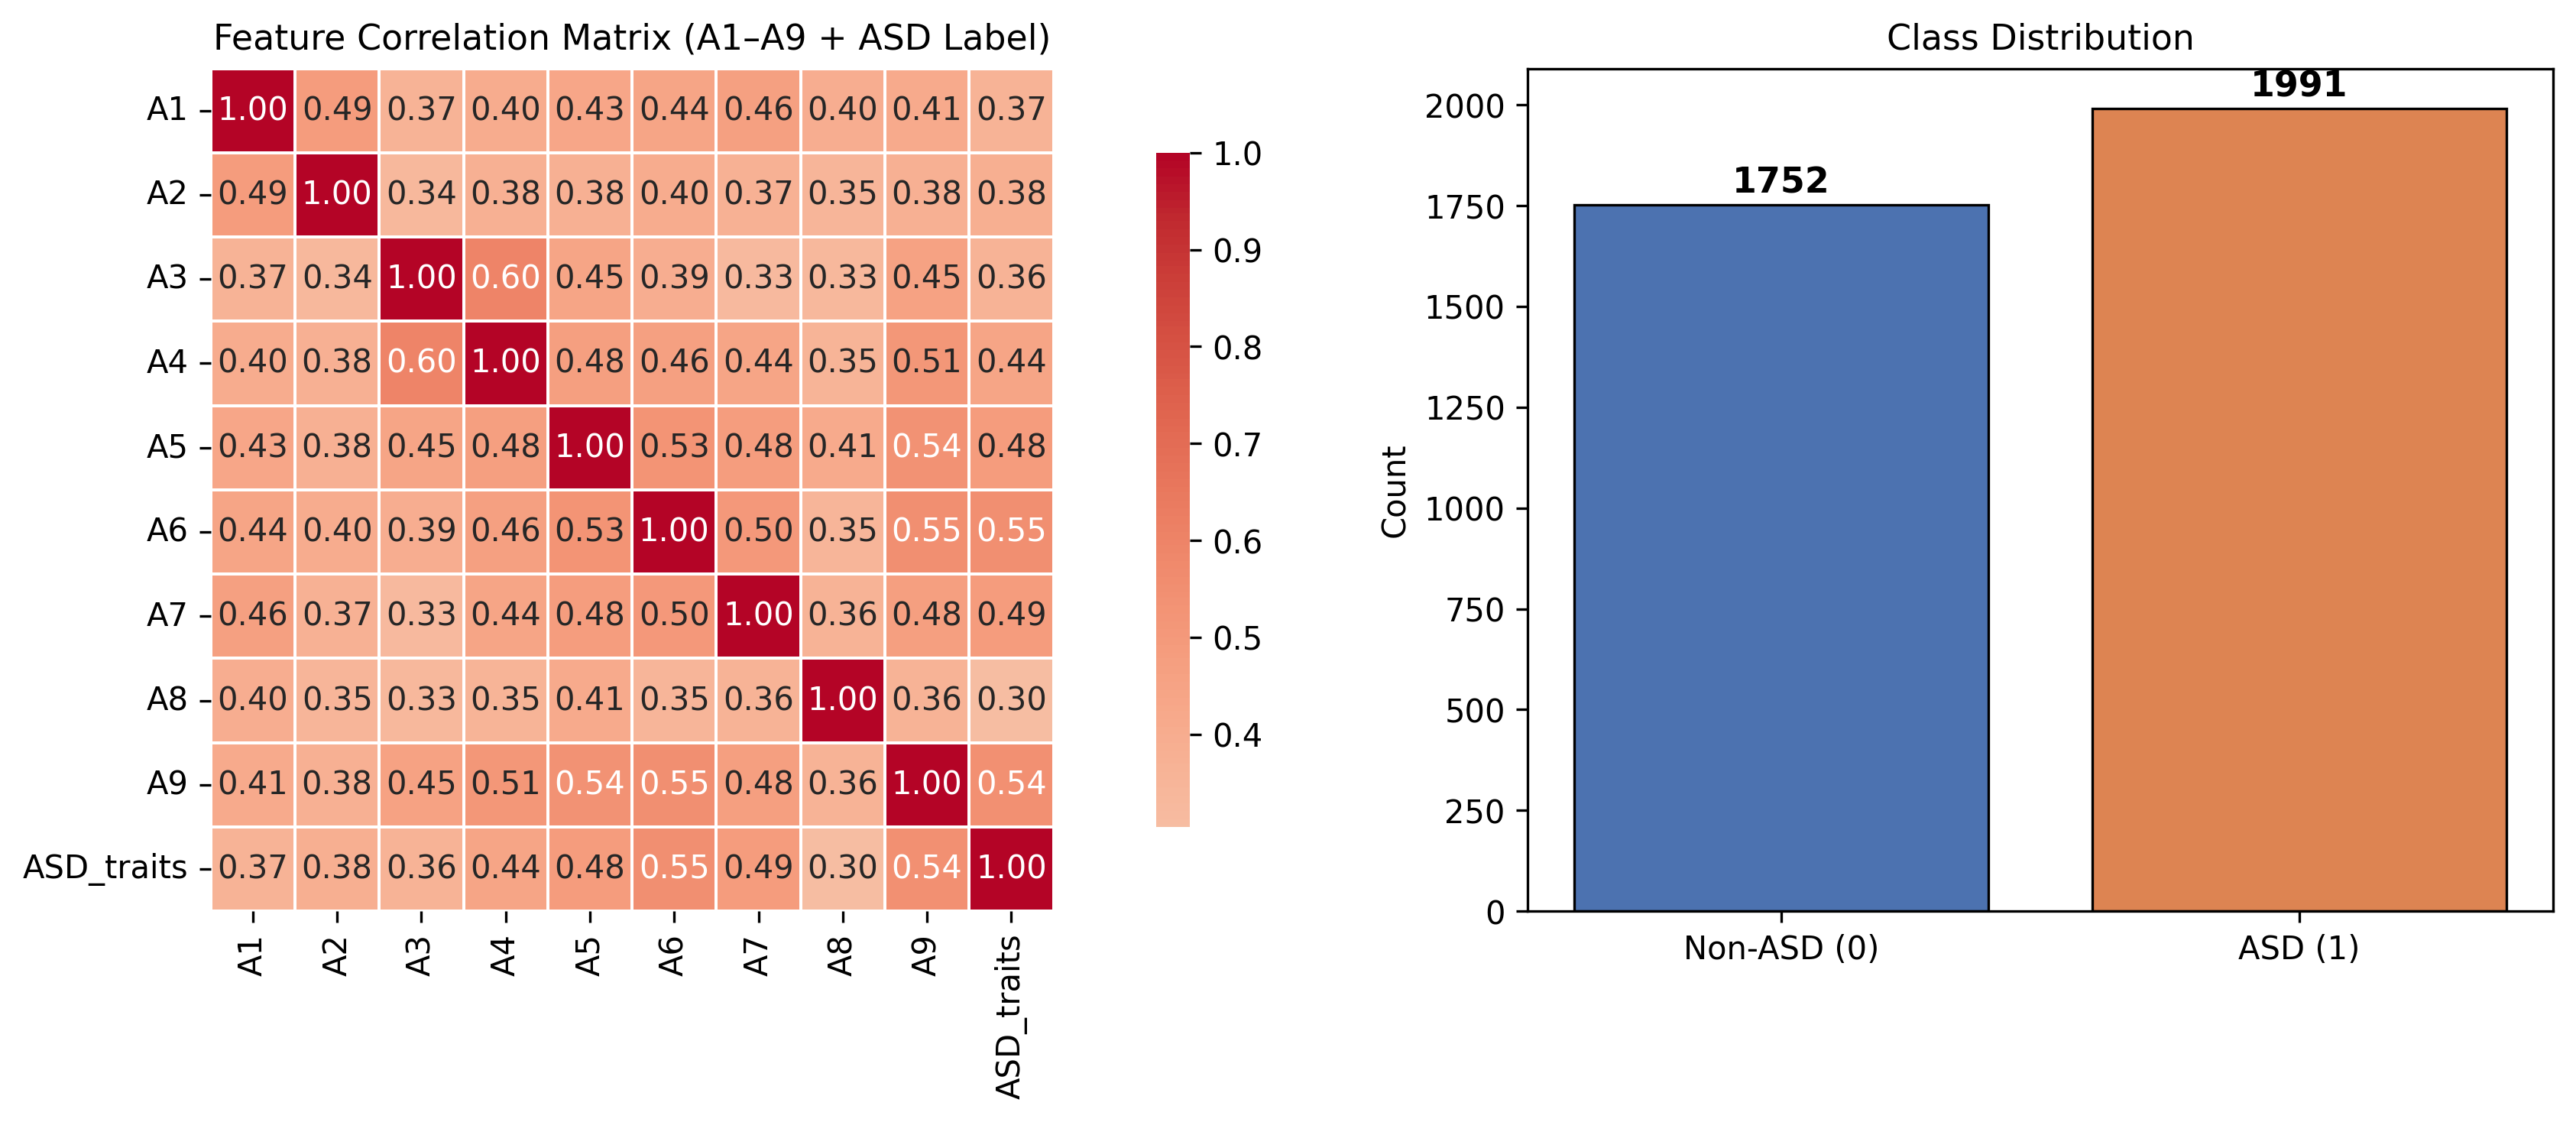
\includegraphics[width=\linewidth]{figures/viz_raw_dataset.png}
\caption{Left: Pearson correlation matrix of clinical questionnaire features (A1--A9) and the ASD target label. Right: class distribution showing 1{,}752 Non-ASD and 1{,}991 ASD instances.}
\label{fig:raw_dataset}
\end{figure}

The nine clinical features (A1--A9) were used across three modelling tracks:
\begin{enumerate}
    \item \textbf{Classical ML (CML):} All nine features were used directly for training classical supervised models.
    \item \textbf{PCA-reduced CML:} Principal Component Analysis was applied to the nine features to obtain a lower-dimensional representation, and classical models were retrained on this reduced feature set.
    \item \textbf{Quantum ML (QML):} The same PCA-reduced representation (4 principal components) was used as input to quantum models, where the reduced features were encoded into qubit rotations via angle encoding before being processed by parameterised quantum circuits.
\end{enumerate}

\subsection{Data Pre-processing}

Data pre-processing was carried out to convert the raw dataset into a form suitable for model training \cite{kotsiantis2006}. The binary questionnaire responses (A1--A9), originally stored as ``YES''/``NO'' strings, were encoded to numerical labels (1/0). Categorical demographic attributes such as sex, ethnicity, and relation were transformed using label-based encoding for mathematical consistency. Numerical features were then normalised using Min-Max Scaling to the range $[0,1]$.

The dataset was split into training (80\%, 2{,}995 instances) and testing (20\%, 749 instances) subsets using stratified sampling to preserve the class distribution of the target variable across both partitions. This single train-test split was applied consistently across all three modelling tracks---CML, PCA-reduced CML, and QML---so that every model was trained and evaluated on the same data partitions, ensuring a fair comparison.

For the PCA-reduced tracks, Principal Component Analysis was fitted on the training set only and then applied to both the training and testing sets. The number of retained components was set to $n=4$, which captures approximately 76\% of the total variance (Fig.~\ref{fig:pca_reduced}, right panel). This choice balances two considerations: (i)~retaining sufficient variance to preserve class-discriminative information, and (ii)~matching the number of qubits available in the quantum circuits, since each principal component is mapped one-to-one to a qubit via angle encoding. Increasing beyond 4~components yields diminishing variance gains (each additional component contributes $<$5\%) while requiring proportionally more qubits, which increases circuit depth, gate count, and simulation cost exponentially. The 4-component, 4-qubit configuration therefore represents a practical trade-off between representational fidelity and near-term quantum hardware constraints.

Figure~\ref{fig:pca_reduced} visualises the PCA-reduced feature space. PC1 alone captures approximately 52\% of the total variance and provides the strongest class separation, while PC2--PC4 contribute an additional 24\% combined with progressively less discriminative power. The scatter plots reveal significant overlap between the ASD and Non-ASD classes even after dimensionality reduction, highlighting the classification challenge faced by all models operating on this representation.

\begin{figure}[!htbp]
\centering
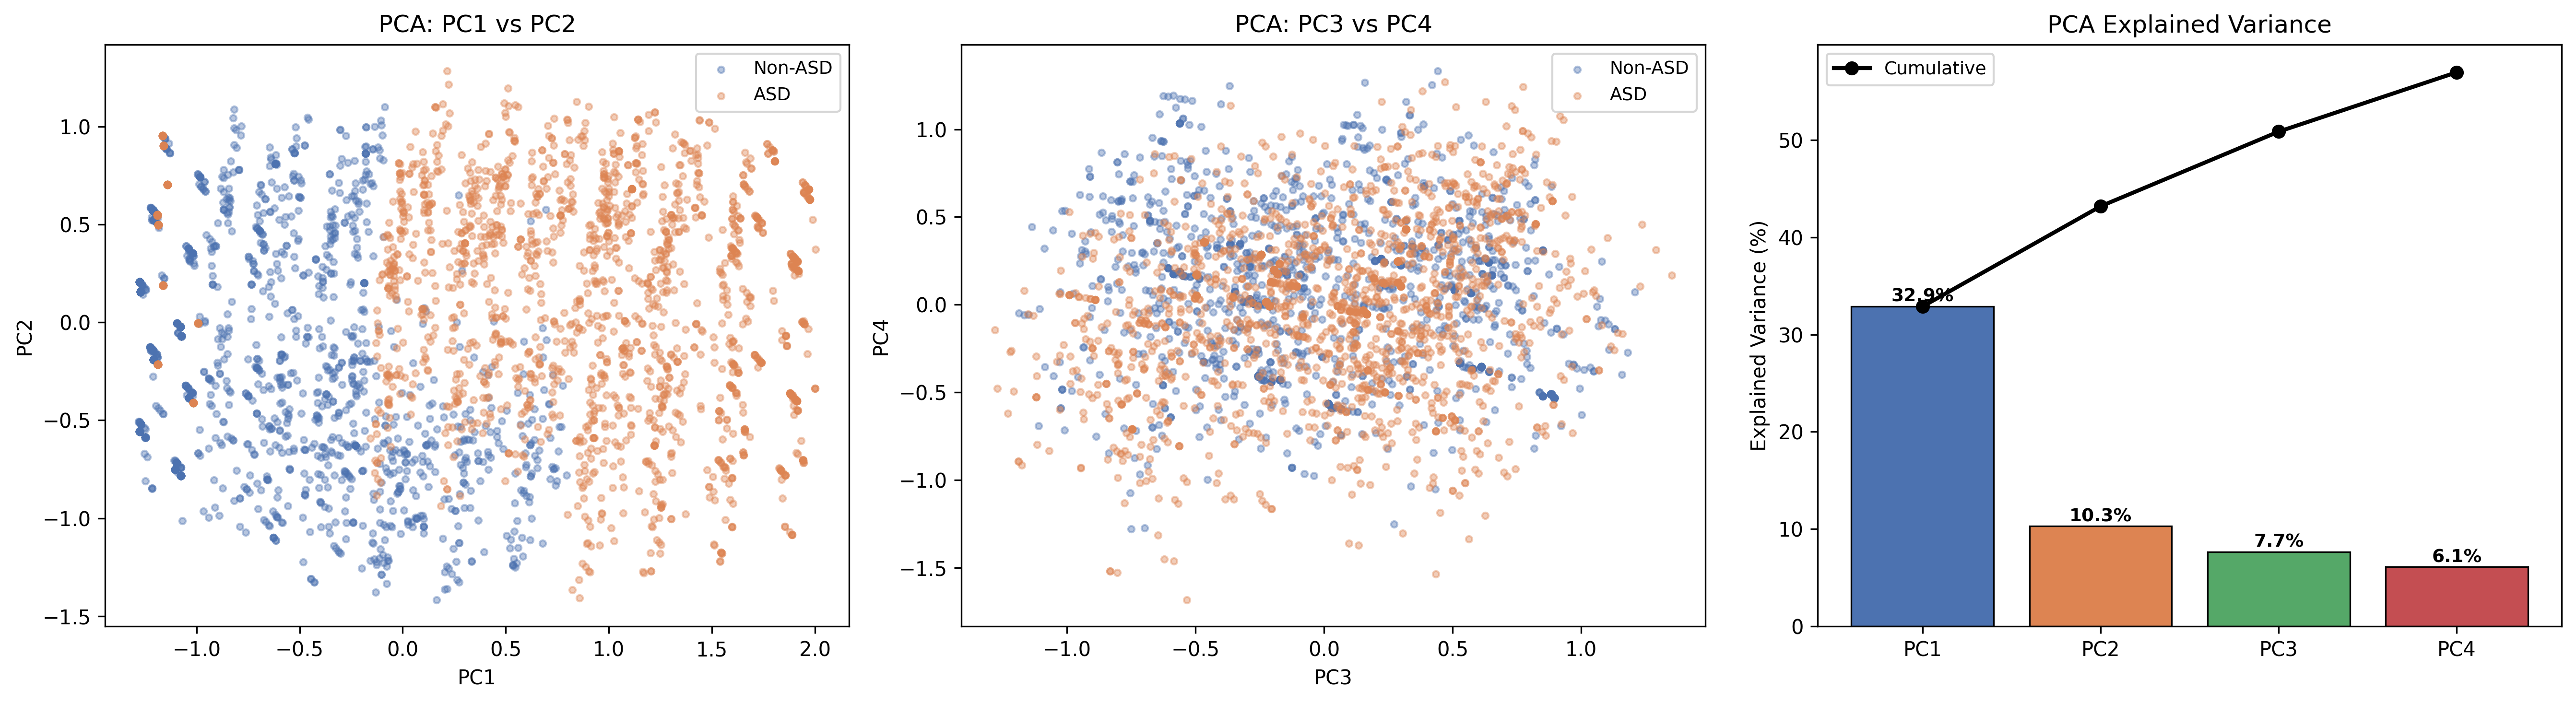
\includegraphics[width=\linewidth]{figures/viz_pca_reduced.png}
\caption{PCA-reduced feature space. Left: PC1 vs PC2 scatter plot coloured by class. Centre: PC3 vs PC4 scatter plot. Right: individual and cumulative explained variance for the four retained principal components.}
\label{fig:pca_reduced}
\end{figure}

\subsection{Exploratory Data Analysis} \label{sec:data_analysis}
Prior to model training, Exploratory Data Analysis (EDA) was conducted on three demographic attributes---ethnicity, sex, and age category---to understand the distribution of ASD traits across different population groups. These demographic features are \emph{not} used as inputs to any of the classification models; they serve solely to characterise the study population and contextualise the prediction results. The nine clinical questionnaire features (A1--A9) are reserved exclusively for the ML and QML pipelines described in the subsequent sections.

\subsubsection{\textbf{Distribution Based on Ethnicity}}
\begin{figure}[ht!]
  \centering
    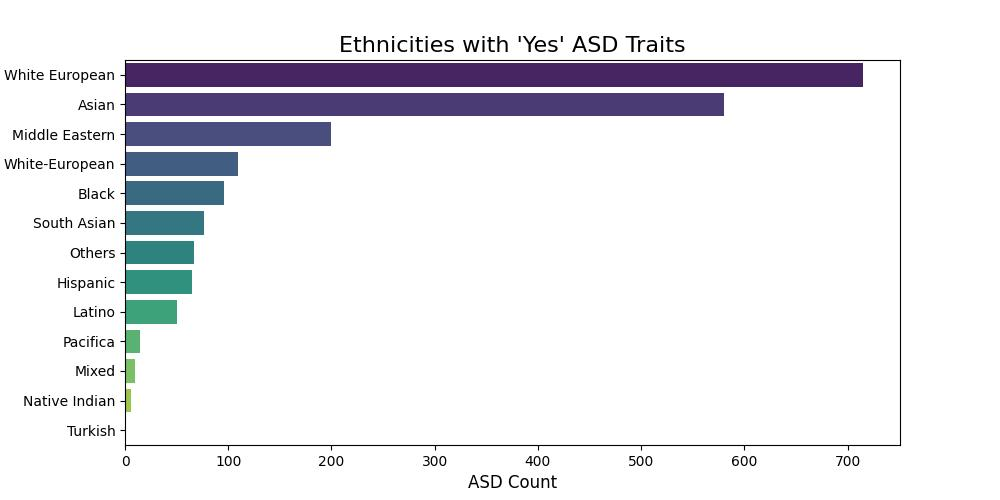
\includegraphics[width=0.9\linewidth]{figures/Ethnicity_yes.jpeg}
    \captionof{figure}{The ethnics with the ASD traits as \enquote{YES}}
    \label{fig:ethni}
\end{figure}
ASD traits were found to be most prevalent in White Europeans within this dataset (\hyperref[fig:ethni]{Fig \ref{fig:ethni}}). This observation could be influenced by various factors, including genetic, social, environmental influences, and potentially higher awareness and access to diagnostic testing in these populations.
\subsubsection{Distribution Based on Sex:}
Analysis indicated that males exhibited ASD traits more frequently than females in this dataset (\hyperref[fig:gen]{Fig \ref{fig:gen}}). Hormonal differences, such as the influence of testosterone on brain development, are often considered as potential contributing factors to this observed gender disparity in ASD prevalence.

\begin{minipage}{0.49\textwidth}
    \centering
    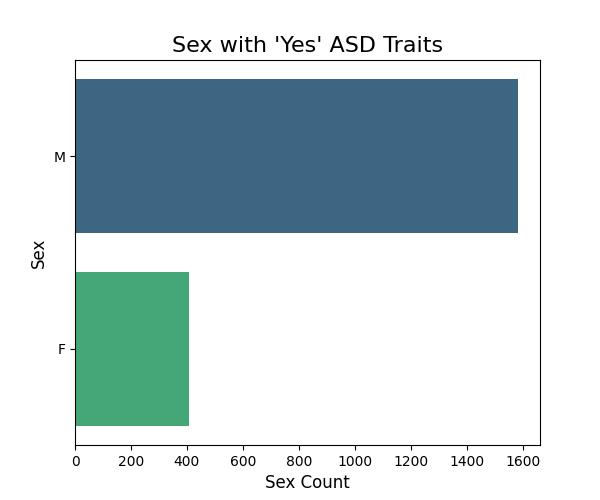
\includegraphics[width=0.99\linewidth]{figures/sex.jpeg}
     \vspace{10pt}
    \captionof{figure}{\centering Gender distribution with ASD traits as \enquote{YES}}
    \label{fig:gen}
\end{minipage}
\hfill
\hfill
\begin{minipage}{0.49\textwidth}
    \centering
     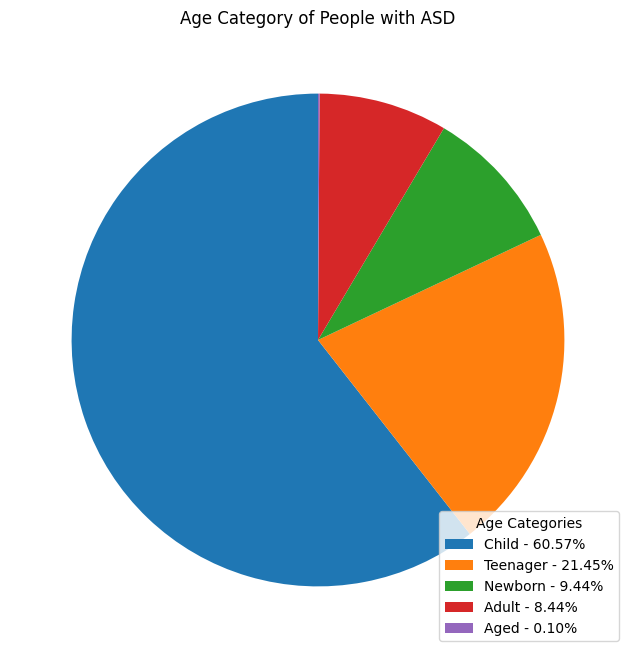
\includegraphics[width=0.9\linewidth]{figures/age_chart.png}
    \captionof{figure}{\centering Age categories distribution of ASD traits:}
    \label{fig:age}
\end{minipage}

\subsubsection{Distribution Based on Age Category}
It was observed that ASD traits were most commonly reported in children, specifically affecting 60.57\% of individuals in the child age category (2-12 years) within the dataset (\hyperref[fig:age]{Fig \ref{fig:age}}, \hyperref[tab:age-category]{Table \ref{tab:age-category}}). This highlights a period of significant susceptibility to exhibiting these traits.

\begin{table}[ht]
   \centering
   \caption{Age Category Traits in Percentage}
   \vspace{0.8em}
   \renewcommand{\arraystretch}{1.3} % Taller rows
   \setlength{\tabcolsep}{20pt}     % Wider columns
   \begin{tabular}{|c|c|}
       \hline
       \textbf{Age Category} & \textbf{Traits (\%)} \\
       \hline
       Newborn & 9.44\% \\
       \hline
       Child & 60.57\% \\
       \hline
       Teenager & 21.45\% \\
       \hline
       Adult & 8.44\% \\
       \hline
       Aged & 0.10\% \\
       \hline
   \end{tabular}
   \label{tab:age-category}
\end{table}

% ---------------------------------------------------------------
% Fix 2: Removed \FloatBarrier before the three QML circuit
%         figures. Changed the enclosing environment from a
%         plain figure[H] (which forced placement and created
%         a gap when the figures did not fit) to figure[!htbp],
%         allowing LaTeX to float the group gracefully to the
%         next page when needed, with no blank space left behind.
% ---------------------------------------------------------------
\subsection{Machine Learning Models Used}\label{sec3.4}
\vspace{-1em}

Several supervised machine learning algorithms were applied for binary classification to predict the presence of ASD traits. 
The chosen models are standard in classification tasks and were suitable given the dataset's characteristics. 
These include Logistic Regression \cite{hosmer2000}, Decision Trees, K-Nearest Neighbors (KNN), 
Na\"{i}ve Bayes, Random Forest \cite{breiman2001}, Support Vector Machine (SVM) \cite{hearst1998}, and 
Histogram Gradient Boosting Classifier (HGBC).
In addition to classical models, we evaluated three Quantum Machine Learning (QML) models, each operating on the 4-component PCA-reduced feature vector. All quantum circuits use 4~qubits, one per principal component. The models differ in their encoding strategy, circuit architecture, and training procedure, as described below.

The foundational step shared by VQC and QNB is angle encoding, where each PCA feature $x_i$ is mapped to a qubit via the rotation $R_Y(\pi \cdot x_i)$. Figure~\ref{fig:quantum_encoding} illustrates this mapping for all four qubits: the horizontal axis shows the PCA feature value and the vertical axis shows the resulting probability $P(|1\rangle) = \sin^2(\pi x_i / 2)$ of measuring the qubit in the $|1\rangle$ state. The sinusoidal encoding introduces a non-linear transformation of the classical features into the quantum Hilbert space, which the subsequent circuit layers (variational ansatz, entanglement, or kernel computation) then exploit for classification.

\begin{figure}[!htbp]
\centering
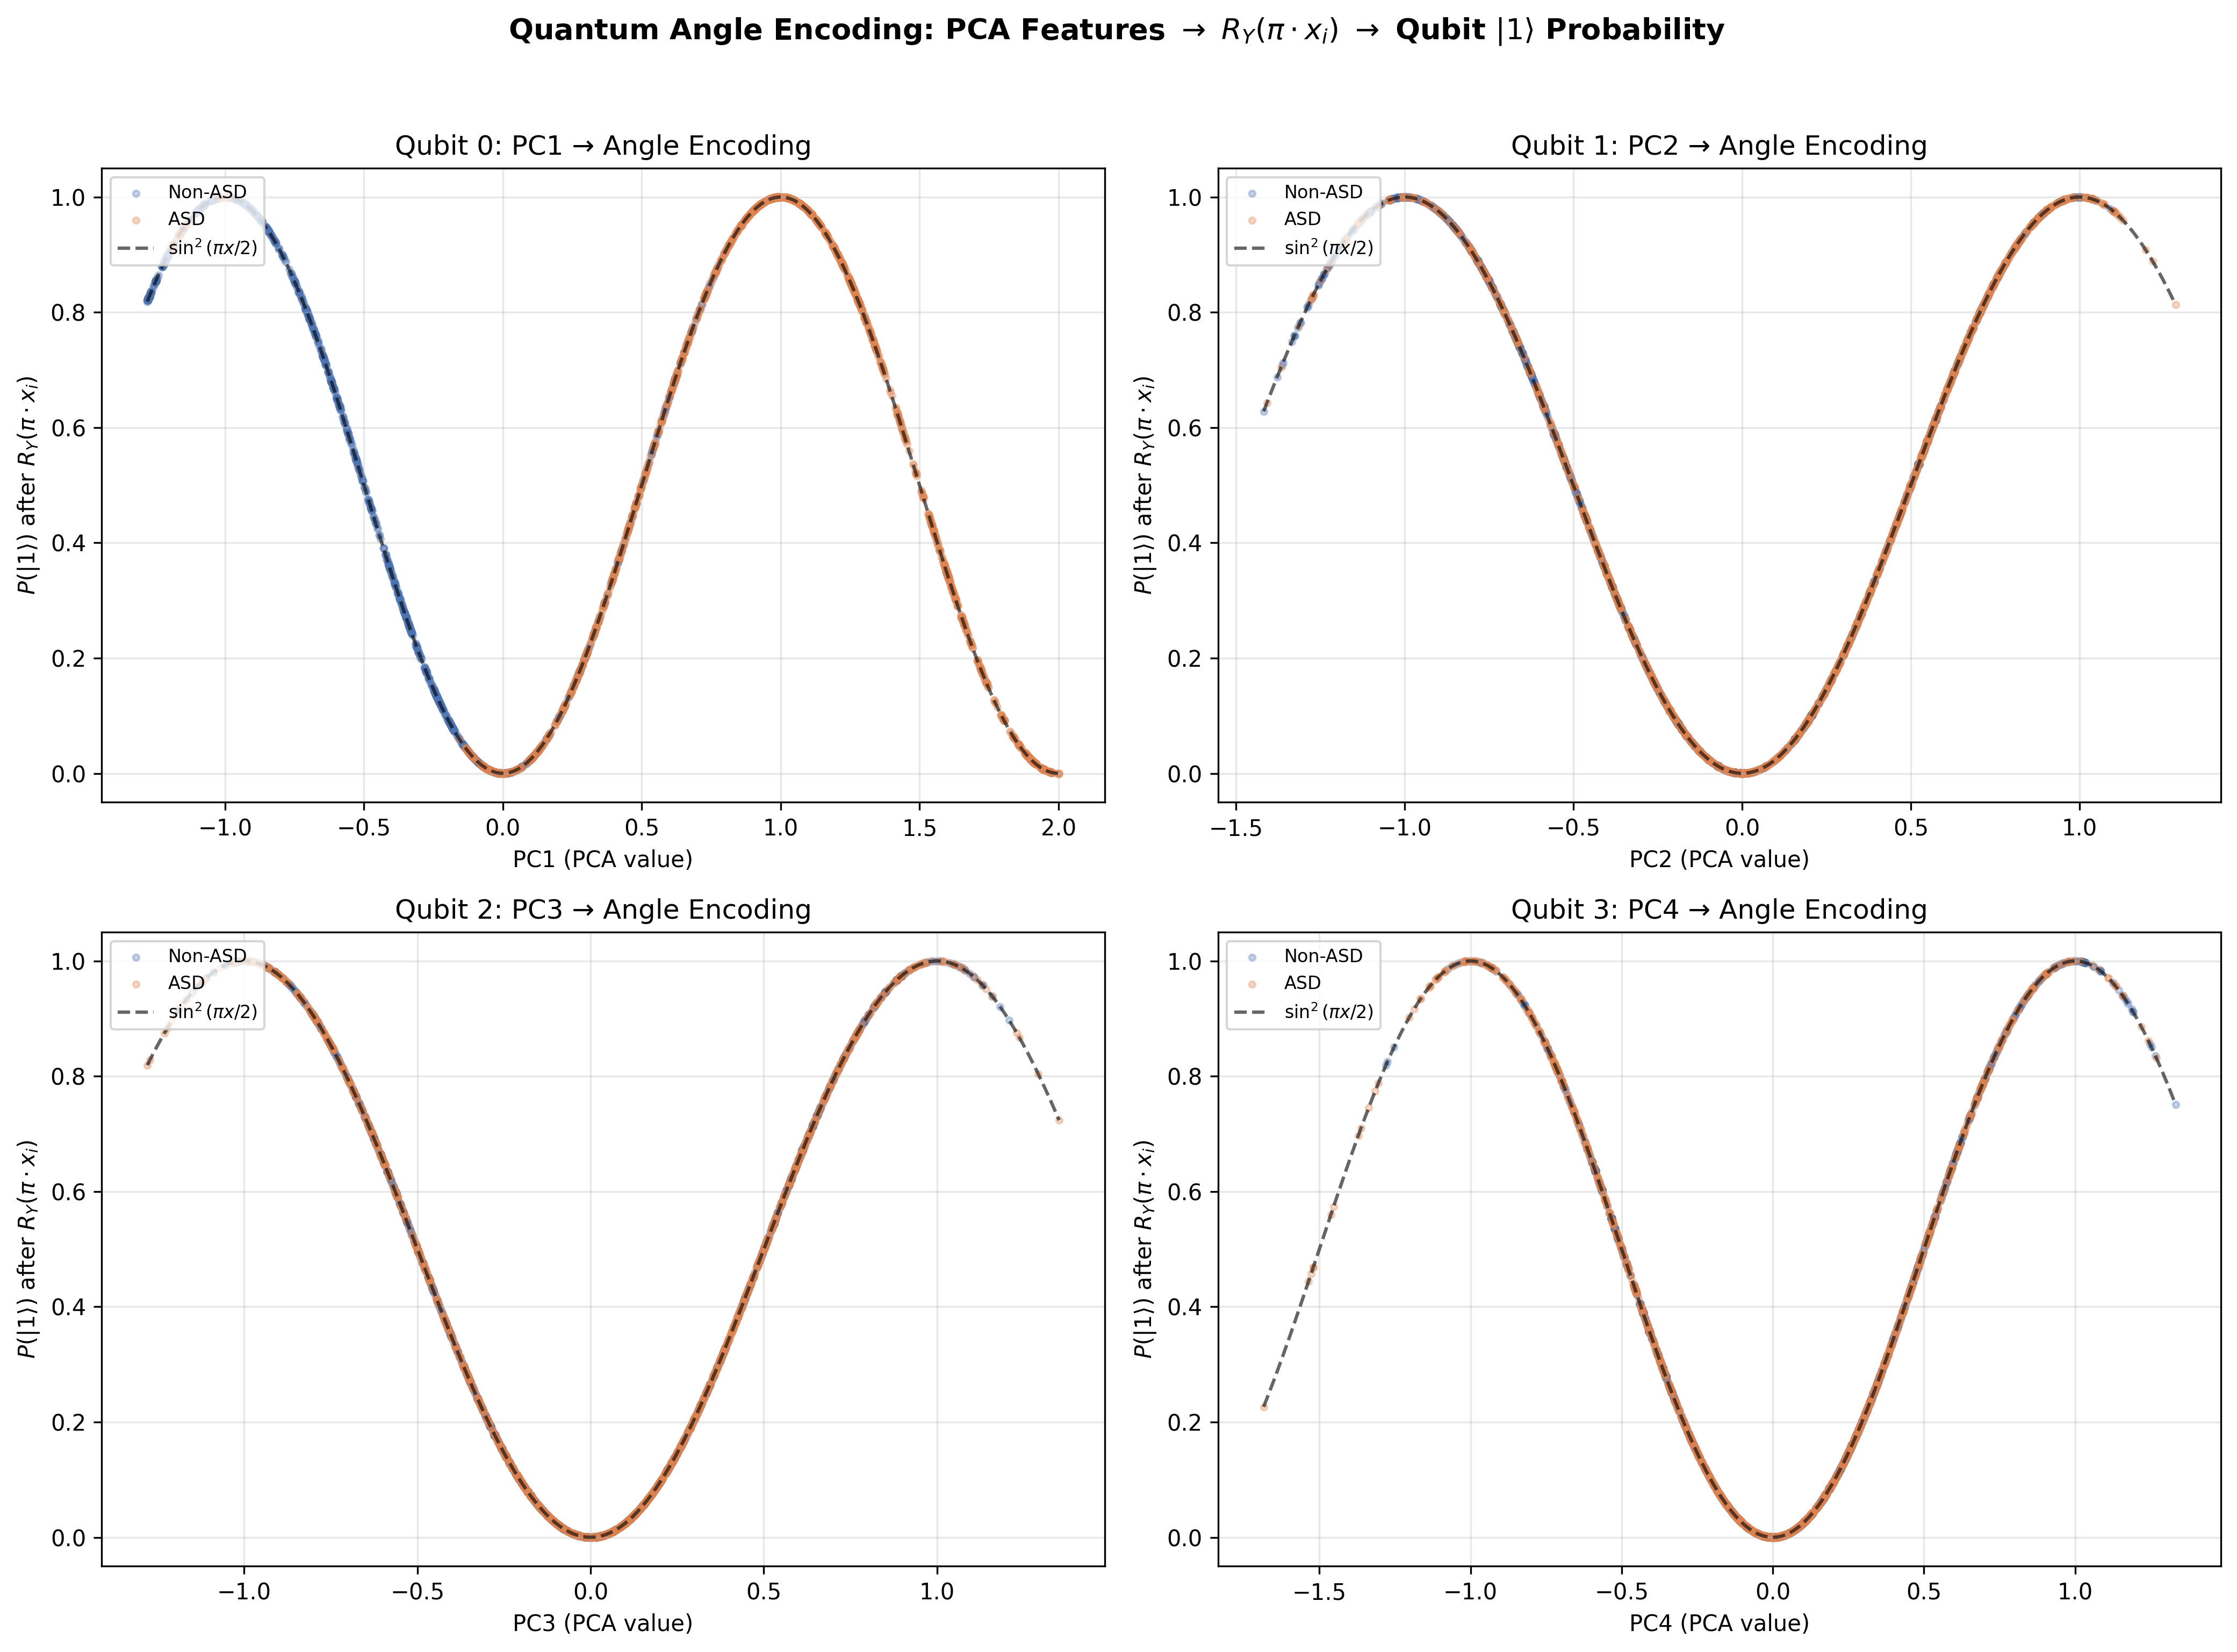
\includegraphics[width=\linewidth]{figures/viz_quantum_encoding.png}
\caption{Quantum angle encoding for each of the four qubits. Each PCA feature value $x_i$ is mapped to the qubit $|1\rangle$ probability via $R_Y(\pi \cdot x_i)$, following the $\sin^2(\pi x / 2)$ curve (dashed). ASD and Non-ASD samples are coloured separately to show class overlap in the encoded space.}
\label{fig:quantum_encoding}
\end{figure}

\subsubsection{Variational Quantum Classifier (VQC)}
\label{sec:vqc}

The VQC \cite{schuld2020} is a hybrid quantum--classical model implemented in PennyLane. The circuit consists of three stages (Fig.~\ref{fig:VQC}):

\paragraph{(i) Angle Encoding.}
Each of the 4~PCA features $x_i \in [0,1]$ is encoded into a qubit via a single-qubit $R_Y$ rotation:
\begin{equation}
R_Y(\pi \cdot x_i)\,|0\rangle \;=\; \cos\!\Bigl(\frac{\pi x_i}{2}\Bigr)|0\rangle \;+\; \sin\!\Bigl(\frac{\pi x_i}{2}\Bigr)|1\rangle
\label{eq:angle_encoding}
\end{equation}
This maps each normalised feature value to the amplitude of a qubit state on the Bloch sphere. A value of $x_i = 0$ leaves the qubit in $|0\rangle$, while $x_i = 1$ rotates it to $|1\rangle$, with intermediate values producing superpositions proportional to the feature magnitude.

\paragraph{(ii) Variational Ansatz.}
A parameterised layer of general single-qubit rotations is applied to each qubit:
\begin{equation}
\text{Rot}(\theta_1, \theta_2, \theta_3) \;=\; R_Z(\theta_3)\,R_Y(\theta_2)\,R_Z(\theta_1)
\end{equation}
This provides 3~trainable parameters per qubit (12~total). Following the rotations, a CNOT ladder ($q_0 \!\to\! q_1 \!\to\! q_2 \!\to\! q_3$) entangles neighbouring qubits, allowing the circuit to capture correlations between encoded features.

\paragraph{(iii) Measurement.}
The expectation value of the Pauli-$Z$ operator on qubit~0 is measured:
\begin{equation}
\hat{y} \;=\; \frac{\langle\psi|Z_0|\psi\rangle + 1}{2} \;\in\; [0,1]
\end{equation}
The raw expectation $\langle Z_0\rangle \in [-1, +1]$ is linearly rescaled to $[0,1]$ to serve as the predicted class probability. A threshold of 0.5 determines the binary classification output.

\paragraph{Training.}
The 12~variational parameters are optimised using the Adam optimiser (learning rate $= 0.1$) over 50~epochs, minimising the mean squared error between the predicted probabilities and the true labels.

\begin{figure}[!htbp]
\centering
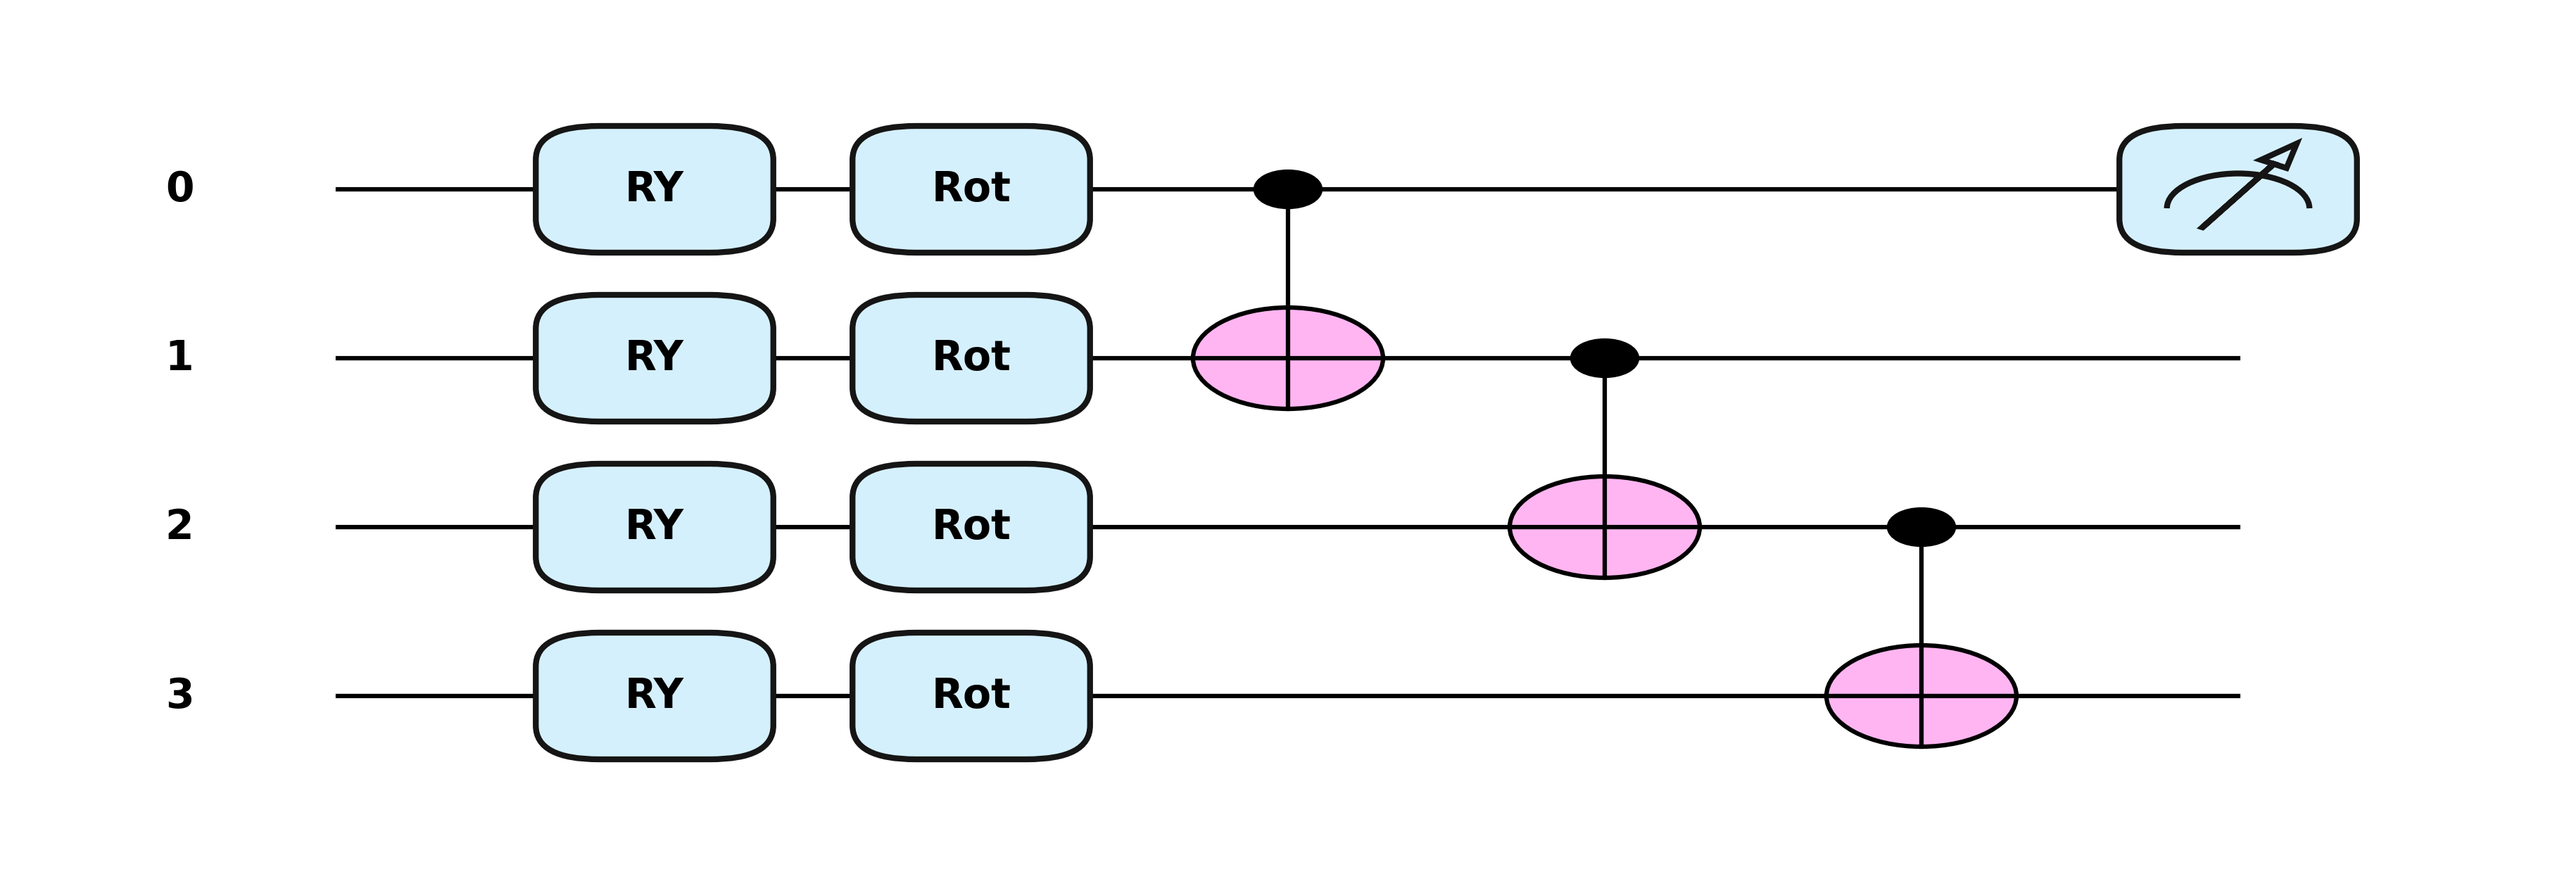
\includegraphics[width=0.7\linewidth]{figures/VQC_circuit.png}
\caption{Quantum circuit for the 4-qubit Variational Quantum Classifier (VQC). Stage~1: $R_Y(\pi x_i)$ angle encoding. Stage~2: $\text{Rot}(\theta_1,\theta_2,\theta_3)$ variational rotations followed by a CNOT entangling ladder. Stage~3: Pauli-$Z$ measurement on qubit~0.}
\label{fig:VQC}
\end{figure}

\subsubsection{Quantum Support Vector Machine (QSVM)}
\label{sec:qsvm}

The QSVM \cite{havlivcek2019} replaces the classical kernel of a Support Vector Machine with a quantum kernel computed from quantum states. Unlike the VQC, the QSVM has \emph{no trainable quantum parameters}; the quantum circuit is used solely to encode data into a high-dimensional Hilbert space, and the classification itself is performed by a classical SVC. The model was implemented using Qiskit with the Aer statevector simulator.

\paragraph{(i) Data Encoding via ZZFeatureMap.}
Each 4-dimensional PCA feature vector $\mathbf{x} = (x_0, x_1, x_2, x_3)$ is encoded into a 4-qubit quantum state using the \texttt{ZZFeatureMap} \cite{havlivcek2019} with 2~repetitions. A single repetition of the map consists of two layers:

\begin{enumerate}
\item \textbf{Single-qubit layer:} A Hadamard gate followed by a $R_Z$ rotation is applied to each qubit:
\begin{equation}
U_{\Phi_i}(x_i) \;=\; R_Z(2\,x_i)\;H
\end{equation}
The Hadamard creates a uniform superposition, and the $R_Z$ rotation imprints the feature value as a phase on qubit~$i$.

\item \textbf{Two-qubit entangling layer:} For every pair of qubits $(i, j)$ with $i < j$, a CNOT--$R_Z$--CNOT sequence encodes pairwise feature interactions:
\begin{equation}
U_{\Phi_{\{i,j\}}} \;=\; \text{CNOT}_{i,j}\;\; R_Z\!\bigl(2\,(\pi - x_i)(\pi - x_j)\bigr)\;\; \text{CNOT}_{i,j}
\end{equation}
This effectively applies the unitary $e^{i\,(\pi - x_i)(\pi - x_j)\,Z_i Z_j}$, entangling pairs of qubits with a phase that depends on the product of their feature values.
\end{enumerate}

With \texttt{reps=2}, this two-layer block is applied twice in succession, increasing the expressibility of the encoding by allowing the quantum state to explore a richer region of the $2^4 = 16$-dimensional Hilbert space.

\paragraph{(ii) Quantum Kernel Computation.}
For each data point $\mathbf{x}$, the feature map produces a quantum state $|\psi(\mathbf{x})\rangle = U_{\Phi}(\mathbf{x})\,|0\rangle^{\otimes 4}$. The statevector is extracted from the simulator and the quantum kernel is defined as the fidelity between pairs of encoded states:
\begin{equation}
K(\mathbf{x}_i, \mathbf{x}_j) \;=\; \bigl|\langle\psi(\mathbf{x}_i)\,|\,\psi(\mathbf{x}_j)\rangle\bigr|^2
\label{eq:quantum_kernel}
\end{equation}
This kernel measures the overlap between two quantum states: if two data points produce similar quantum states, their kernel value is close to~1; if they map to nearly orthogonal states, the value approaches~0. This is analogous to the classical kernel trick, but the mapping is into a Hilbert space whose dimension grows exponentially with the number of qubits.

\paragraph{(iii) Classical SVM Classification.}
The full kernel matrix $K_{ij}$ is precomputed for all training and test samples, and a classical SVC with \texttt{kernel="precomputed"} is trained on the quantum kernel matrix. The SVM finds the optimal separating hyperplane in the quantum feature space without ever explicitly constructing the high-dimensional feature vectors.

\begin{figure}[H]
\centering
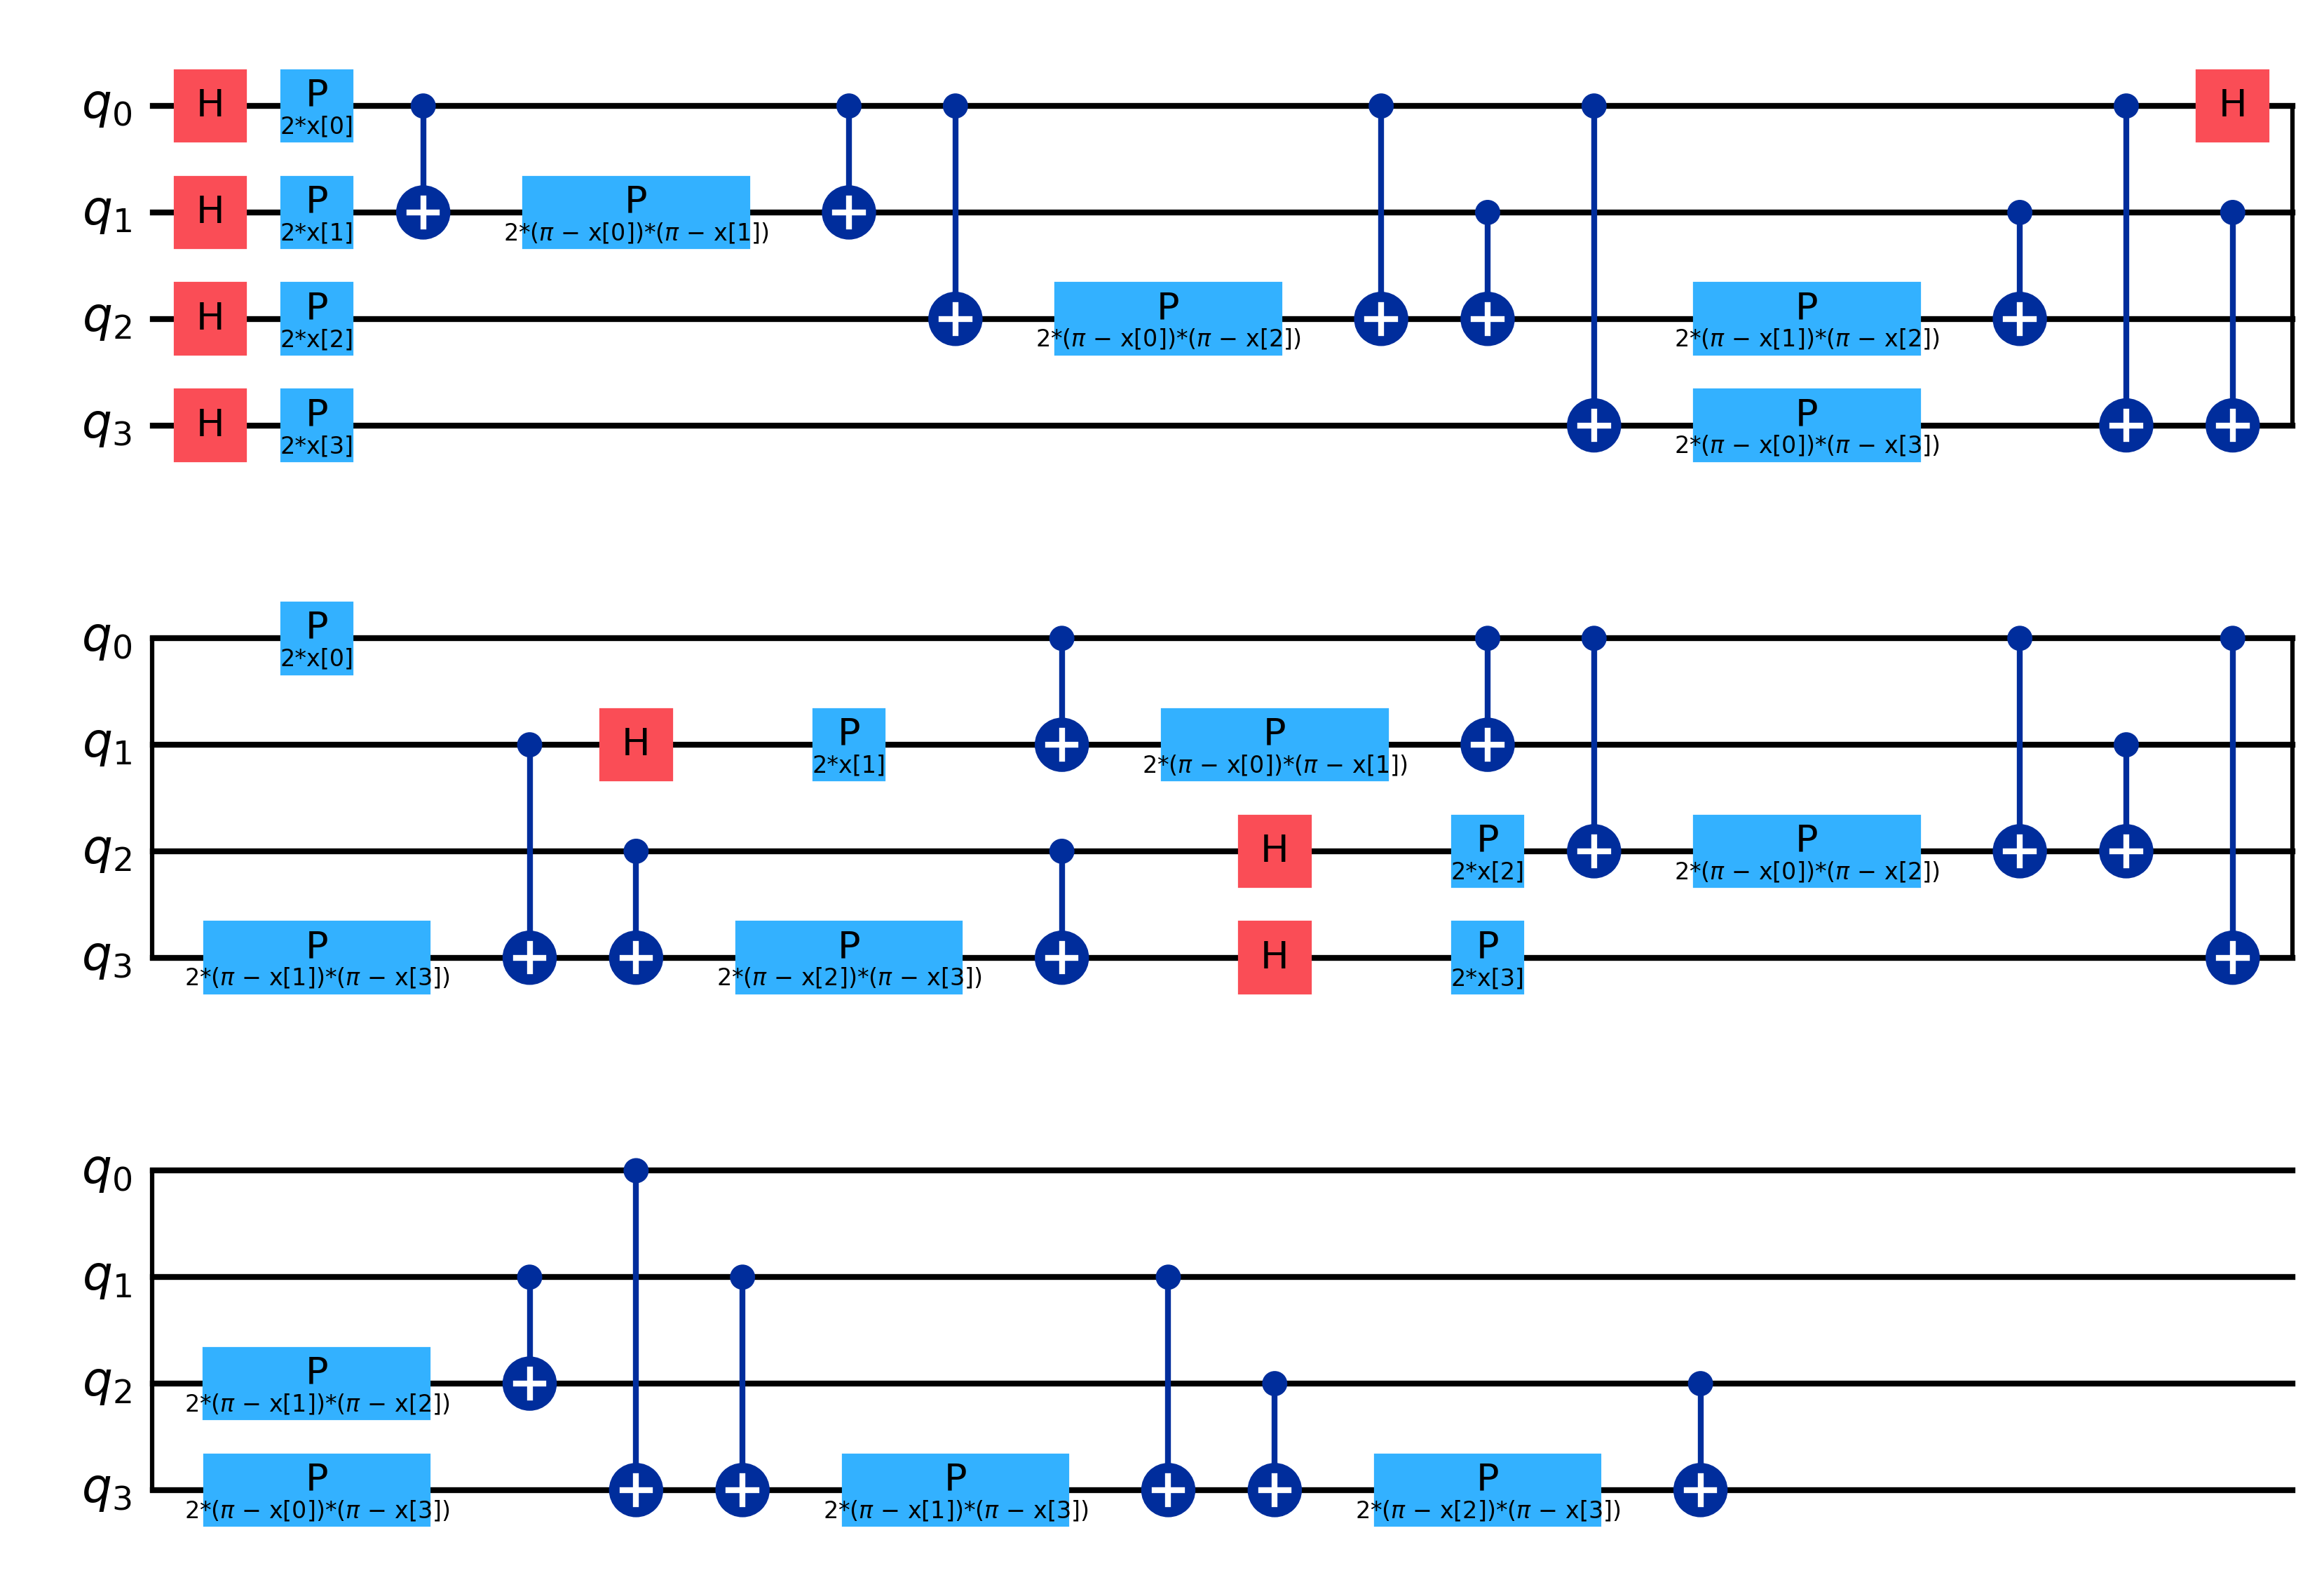
\includegraphics[width=0.85\linewidth]{figures/QSVM_circuit.png}
\caption{Quantum circuit for the ZZFeatureMap ($\text{reps}=2$) used in the QSVM. Each repetition applies $H$--$R_Z(2x_i)$ on each qubit, followed by CNOT--$R_Z(2(\pi-x_i)(\pi-x_j))$--CNOT entangling gates on all qubit pairs. The output statevector is used to compute the fidelity kernel.}
\label{fig:QSVM}
\end{figure}

\subsubsection{Quantum Naive Bayes (QNB)}
\label{sec:qnb}

The Quantum Naive Bayes (QNB) model is a hybrid quantum-classical classifier that uses a parameterless quantum circuit as a non-linear feature transformer, whose outputs are then classified by a classical Gaussian Naive Bayes estimator. Unlike VQC, the quantum circuit contains \emph{no trainable parameters}; unlike QSVM, it does not compute a kernel matrix but instead produces transformed feature vectors directly. The circuit employs \emph{data re-uploading}~\cite{perez2020} with \emph{multi-scale encoding}, repeating the encoding--entanglement block $L=6$ times with layer-dependent scaling factors to increase expressivity, and measures the full $2^4=16$-dimensional probability distribution rather than individual qubit expectations.

\paragraph{Encoding--Entanglement Block.}
Each of the $L=6$ layers applies three sub-stages in sequence with a layer-dependent scale factor $s_\ell = \ell$ (for $\ell = 1,\ldots,6$). First, amplitude encoding via $R_Y$ rotations:
\begin{equation}
U_{\text{amp}}^{(\ell)} = \bigotimes_{i=0}^{3} R_Y(\pi \cdot x_i \cdot s_\ell),
\end{equation}
followed by a CNOT ring that entangles all four qubits with wrap-around connectivity:
\begin{equation}
U_{\text{ent}} = \text{CNOT}_{3 \to 0} \cdot \text{CNOT}_{2 \to 3} \cdot \text{CNOT}_{1 \to 2} \cdot \text{CNOT}_{0 \to 1},
\end{equation}
and finally phase encoding via $R_Z$ rotations at the same scale:
\begin{equation}
U_{\text{phase}}^{(\ell)} = \bigotimes_{i=0}^{3} R_Z(\pi \cdot x_i \cdot s_\ell).
\end{equation}
The ring topology ensures that every qubit is entangled with its neighbours, enabling the circuit to capture pairwise feature interactions that a classical Naive Bayes model (which assumes feature independence) cannot represent on its own. The multi-scale factors $(1\times, 2\times, \ldots, 6\times)$ cause each re-uploading layer to encode the data at a different frequency, creating a Fourier-like expansion in Hilbert space that increases the circuit's representational capacity beyond uniform re-uploading.

\paragraph{Measurement.}
After all $L$ layers, the circuit measures the computational-basis probability distribution:
\begin{equation}
p_j = |\langle j | \psi \rangle|^2, \quad j \in \{0,\ldots,15\},
\end{equation}
yielding a 16-dimensional feature vector $\mathbf{p} = (p_0, \ldots, p_{15})$ for each input sample. This is exponentially richer than the 4 expectation values used in VQC, providing the downstream classifier with a high-resolution fingerprint of the quantum state.

\paragraph{Classical Classification.}
The probability vectors $\{\mathbf{p}^{(k)}\}$ are passed to a Gaussian Naive Bayes (GNB) classifier, which models each class-conditional distribution as $p(\mathbf{p} \mid y) = \prod_{j} \mathcal{N}(p_j;\, \mu_{y,j},\, \sigma^2_{y,j})$ and applies Bayes' rule for prediction. The quantum circuit thus acts as a non-linear feature map that introduces inter-feature entanglement, compensating for the conditional-independence assumption of classical NB.

The QNB pipeline requires no iterative training of quantum parameters—only a single forward pass through the circuit per sample—making it significantly faster than VQC while still leveraging quantum feature transformations. The implementation uses PennyLane with the same $R_Y$ angle encoding as VQC, and the circuit structure is shown in Figure~\ref{fig:QNB}.

\begin{figure}[H]
\centering
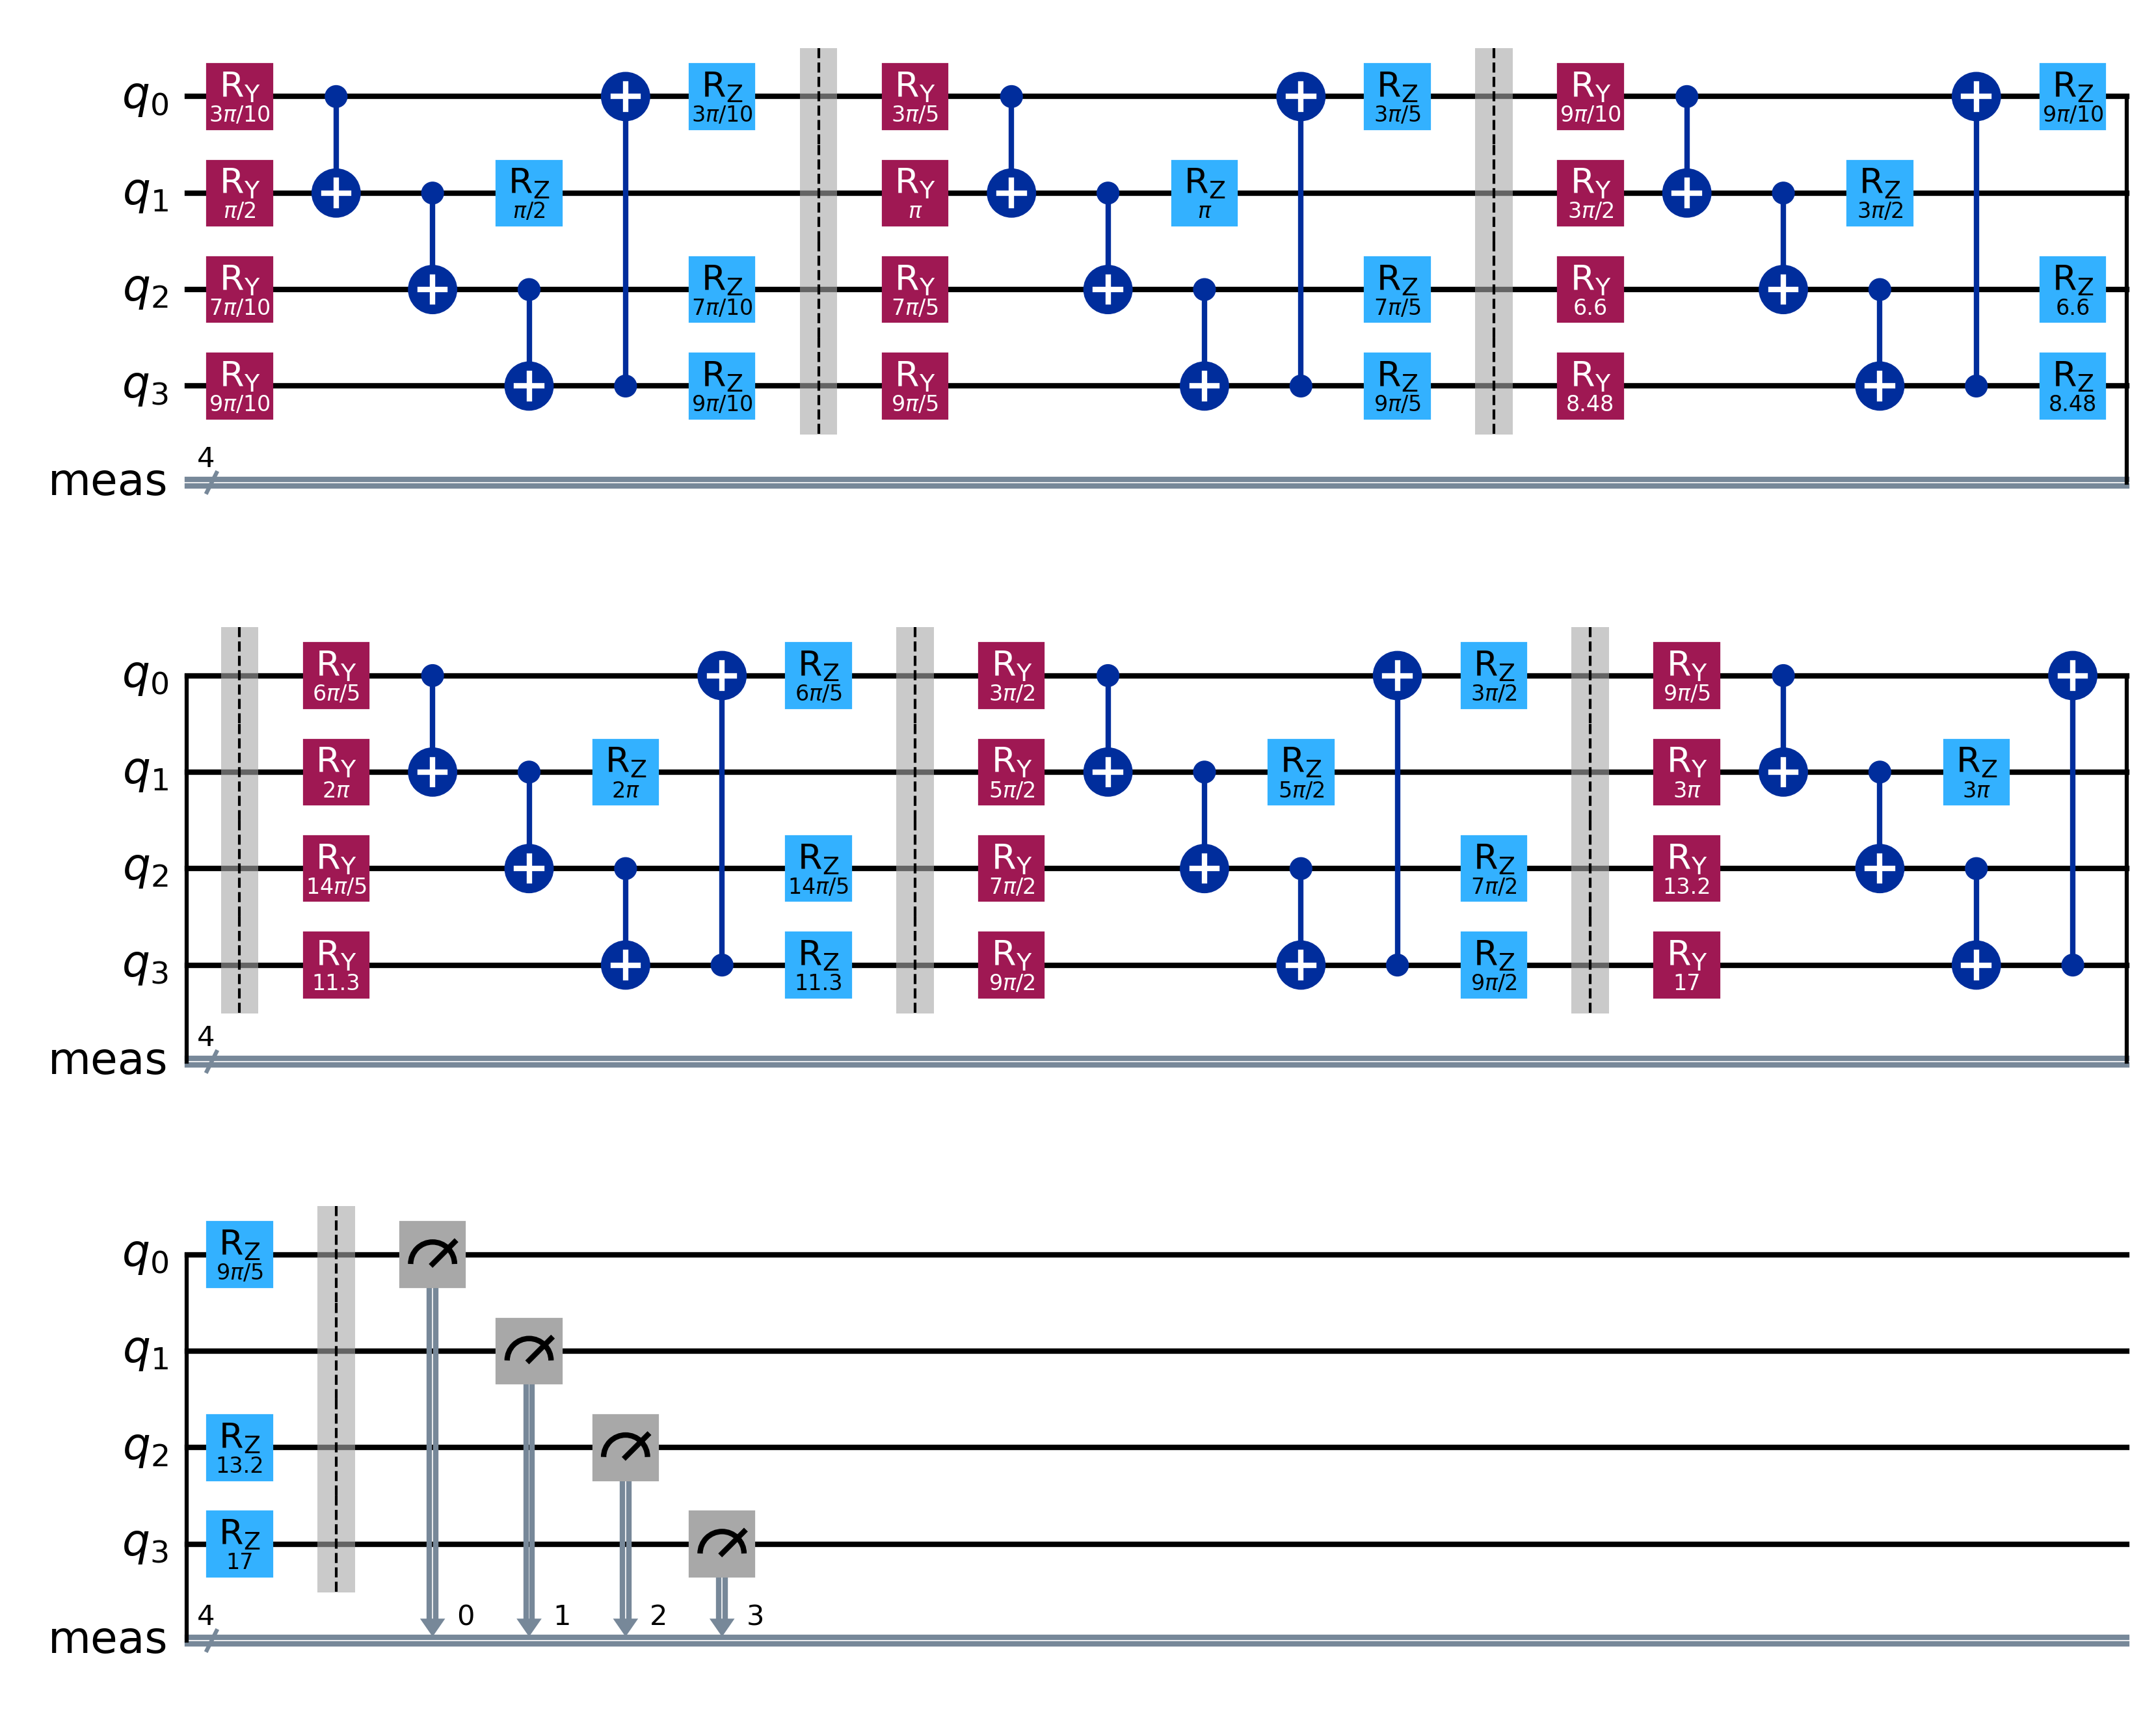
\includegraphics[width=0.85\linewidth]{figures/QNB_circuit.png}
\caption{Quantum circuit for the Quantum Naive Bayes (QNB) model. Each of the $L=6$ data re-uploading layers applies $R_Y(\pi \cdot x_i \cdot s_\ell)$ amplitude encoding, a CNOT ring for entanglement, and $R_Z(\pi \cdot x_i \cdot s_\ell)$ phase encoding with multi-scale factors $s_\ell = 1,\ldots,6$. The final measurement yields a 16-dimensional probability vector fed to a classical Gaussian Naive Bayes classifier.}
\label{fig:QNB}
\end{figure}

\section{Performance Analysis}\label{sec4}

The predictive performance of all classical and quantum classification models was evaluated using standard metrics. Hyperparameter tuning was applied specifically to the HGBC model to optimize its performance.

\subsection{Hyperparameter Tuning and Confusion Matrix Analysis}\label{sec:hptuning}

\subsubsection{Hyperparameter Tuning for Classical Models}
For the Histogram Gradient Boosting Classifier (HGBC), hyperparameter tuning was conducted using grid search with cross-validation to identify optimal settings for maximizing accuracy. The hyperparameters explored were: number of estimators, learning rate, maximum iterations, maximum depth, minimum samples per leaf, and L2 regularisation strength.

The top~10 hyperparameter combinations and their corresponding mean test accuracies are summarised in Table~\ref{tab:hparam_combos} and visualised in Fig.~\ref{fig:bestparameter}.

\begin{table}[ht]
\centering
\caption{Top 10 Hyperparameter Combinations for HGBC}
\label{tab:hparam_combos}
\renewcommand{\arraystretch}{1.15}
\setlength{\tabcolsep}{3pt}
\begin{tabular}{|c|c|c|c|c|c|c|c|}
\hline
\textbf{ID} & \textbf{L2 Reg.} & \textbf{LR} & \textbf{Max Depth} & \textbf{Max Iter} & \textbf{Min Leaf} & \textbf{Accuracy (\%)} \\
\hline
C1  & 1.0 & 0.2  & 10 & 100 & 30 & 97.15 \\
C2  & 1.0 & 0.1  & 10 & 100 & 30 & 97.07 \\
C3  & 1.0 & 0.05 & 10 & 300 & 30 & 97.02 \\
C4  & 1.0 & 0.2  & 10 & 300 & 30 & 97.01 \\
C5  & 1.0 & 0.1  & 10 & 200 & 30 & 96.99 \\
C6  & 1.0 & 0.2  & 10 & 200 & 30 & 96.96 \\
C7  & 1.0 & 0.2  & 10 & 300 & 30 & 96.94 \\
C8  & 0.0 & 0.1  & 10 & 200 & 30 & 96.91 \\
C9  & 1.0 & 0.2  & 10 & 200 & 10 & 96.90 \\
C10 & 1.0 & 0.05 & 10 & 300 & 20 & 96.89 \\
\hline
\end{tabular}
\end{table}

\begin{figure}[ht]
    \centering
    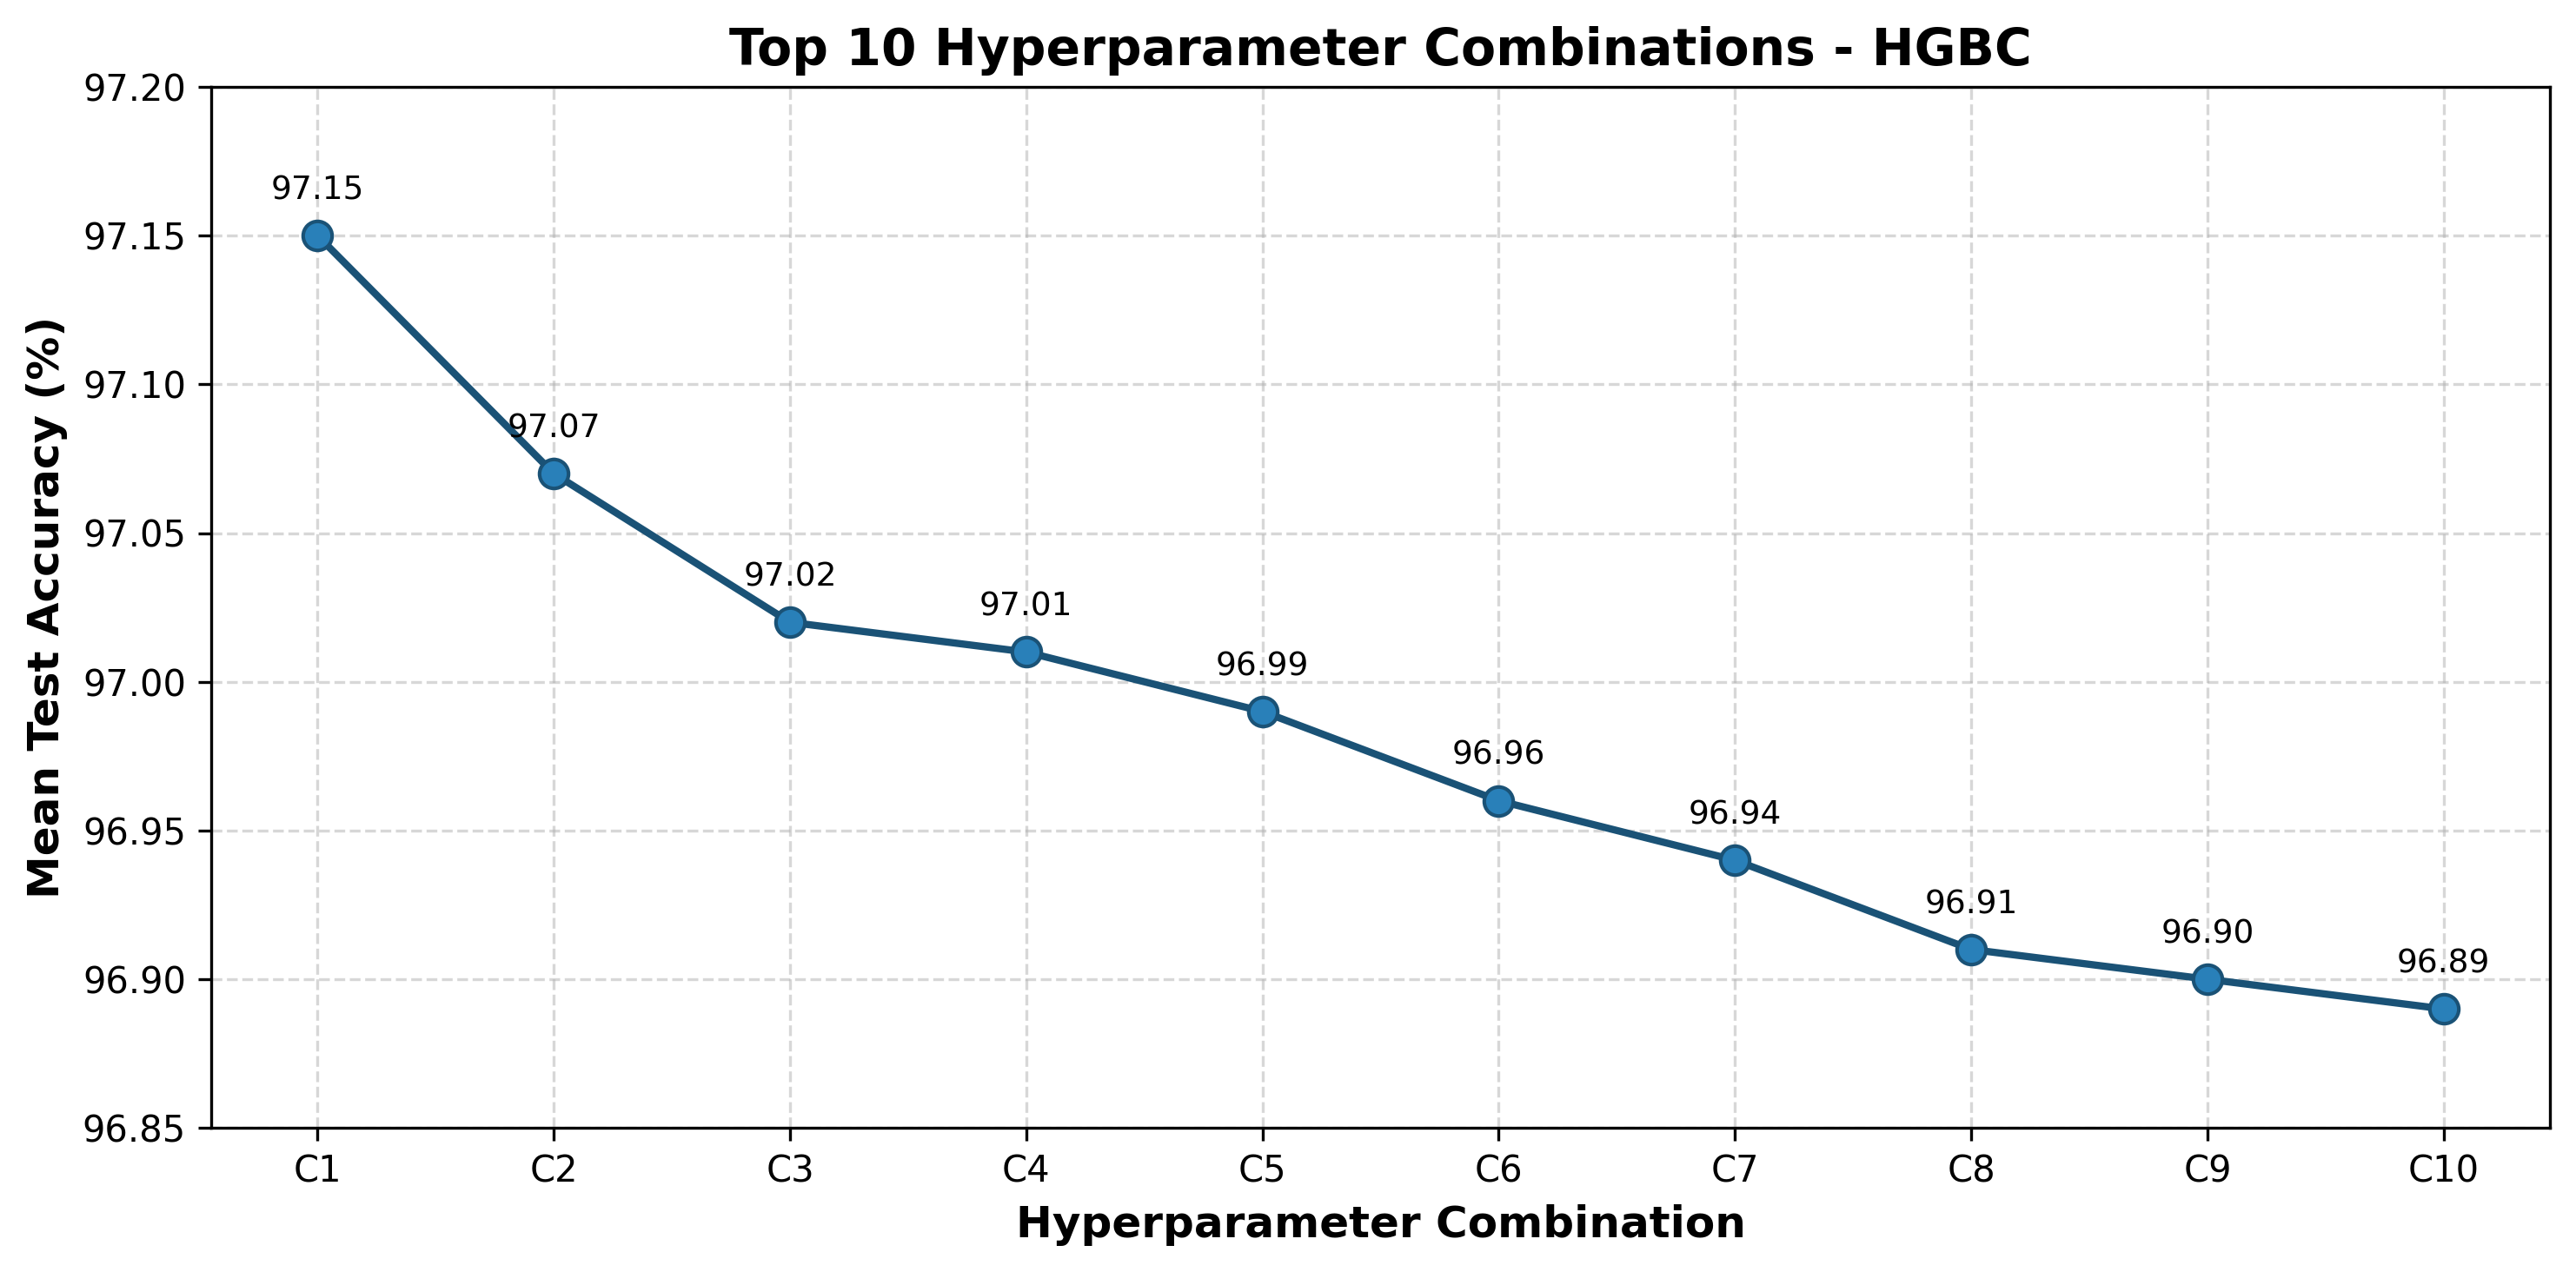
\includegraphics[width=0.9\linewidth]{figures/hyperparameter_combination_line.png}
    \caption{Mean test accuracy for the top~10 hyperparameter combinations (C1--C10) of HGBC, as defined in Table~\ref{tab:hparam_combos}.}
    \label{fig:bestparameter}
\end{figure}

The best-performing configuration (C1) achieved a mean test accuracy of approximately 97.15\% with a maximum depth of~10, minimum samples per leaf of~30, and a learning rate of~0.2. The strong performance of HGBC on this dataset can be attributed to its histogram-based binning strategy, which discretises continuous features into a fixed number of bins, reducing the computational cost of split finding from $O(N)$ to $O(B)$ where $B \ll N$ is the number of bins. This binning also acts as an implicit regulariser, preventing the model from overfitting to noise in individual feature values. Additionally, the combination of moderate tree depth (10) and a relatively high minimum leaf size (30) constrains model complexity, ensuring that each leaf node captures a statistically meaningful number of samples rather than memorising isolated instances. The L2 regularisation further penalises large leaf weights, contributing to better generalisation. These factors together allow HGBC to capture the non-linear interactions among the nine binary questionnaire features while maintaining robustness on unseen data.

\subsubsection{Confusion Matrix Analysis: Classical Models}
The confusion matrix summarizes model performance by counting 
True Positives, True Negatives, False Positives, False Negatives.

Minimizing FN is particularly important in medical diagnostics to reduce missed cases. Table~\ref{tab:algorithm_metrics} shows the confusion matrix counts for different classical models.  

\begin{table}[ht]
\centering
\caption{Confusion Matrix Metrics of Classical Machine Learning Models}
\label{tab:algorithm_metrics}
\begin{tabular}{lrrrr}
        \toprule
        \textbf{Algorithm} & \textbf{TN} & \textbf{FP} & \textbf{FN} & \textbf{TP} \\
        \midrule
        Logistic Regression (LR) & 274 & 65 & 84 & 326 \\
        Naive Bayes (NB) & 306 & 43 & 68 & 332 \\
        Decision Tree (DT, log-loss) & 312 & 27 & 20 & 390 \\
        K-Nearest Neighbor (KNN, Euclidean) & 330 & 19 & 26 & 374 \\
        SVM (RBF) & 334 & 15 & 7 & 393 \\
        Random Forest (RF) & 337 & 12 & 18 & 382 \\
        Histogram Gradient Boosting (HGBC) & 343 & 6 & 10 & 390 \\
        \bottomrule
\end{tabular}
\end{table}

\subsubsection{Confusion Matrix Analysis: Quantum Machine Learning Models}
Similarly, we analyzed the confusion matrices for our quantum machine learning (QML) models---VQC, QSVM, and QNB---using PCA-reduced features. Although QML models show promise in handling overlapping and high-dimensional datasets, their performance in our experiments was lower than classical ensemble methods, due to shallow circuit architectures and the limited expressivity of 4-qubit systems operating on PCA-reduced features. Table~\ref{tab:qml_metrics} summarizes the confusion matrix counts for QML models.


\begin{table}[ht]
\centering
\caption{Confusion Matrix Metrics of Quantum Machine Learning Models (PCA-Reduced)}
\label{tab:qml_metrics}
\begin{tabular}{lrrrr}
\toprule
\textbf{Algorithm} & \textbf{TN} & \textbf{FP} & \textbf{FN} & \textbf{TP} \\
\midrule
VQC  & 256 & 95 & 243 & 155 \\
QSVM & 244 & 107 & 63 & 335 \\
QNB  & 207 & 144 & 131 & 267 \\
\bottomrule
\end{tabular}
\end{table}

This section highlights the clear separation in performance between classical ensemble approaches (RF, HGBC) and quantum models (QSVM, VQC, QNB). While quantum approaches have potential, deeper circuits, more qubits, and richer feature encodings may be required to match classical methods on this dataset. All three quantum models were evaluated on the same PCA-reduced test set (749 samples) using the identical 80/20 stratified split \cite{bishop2006}.

The quantum machine learning models used in this study are illustrated in the diagrams. Figure~\ref{fig:VQC} shows the circuit structure of the Variational Quantum Classifier implemented with a four-qubit variational ansatz. Figure~\ref{fig:QSVM} represents the quantum feature map and kernel circuit used in the Quantum Support Vector Machine model. Figure~\ref{fig:QNB} illustrates the hybrid quantum-classical circuit used in the Quantum Naive Bayes approach.

\subsection{Precision and Recall of Classical Models}\label{sec:precision_recall}


Precision (TP / (TP + FP)) and Recall (TP / (TP + FN)) are critical metrics for evaluating the model's ability to correctly identify positive cases and avoid false positives. Graphical representations are provided for illustration.

\begin{figure}[h!]
    \centering
    \begin{minipage}{0.48\textwidth}
        \centering
        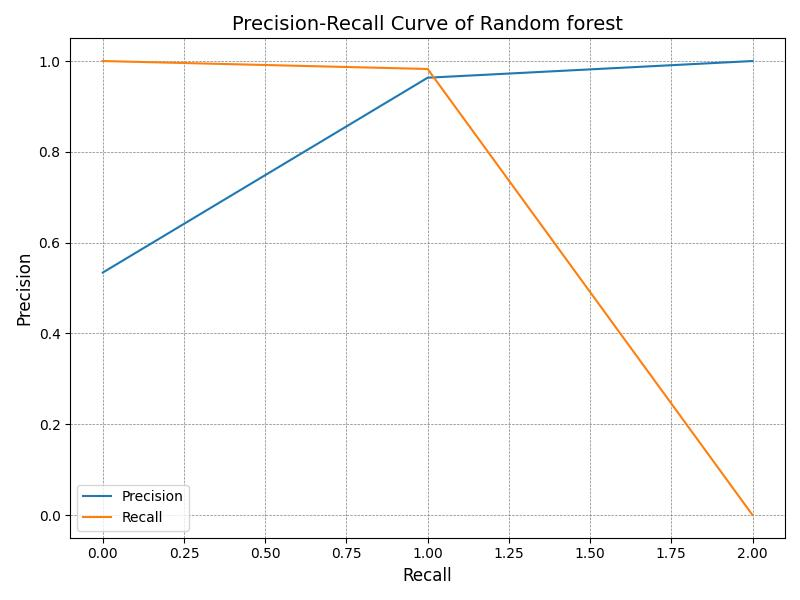
\includegraphics[width=0.95\linewidth]{figures/pre_re_rf.jpeg}
        \captionof{figure}{Precision and Recall: RF}
        \label{fig:pre-re-rf}
    \end{minipage}
    \hfill
    \begin{minipage}{0.48\textwidth}
        \centering
        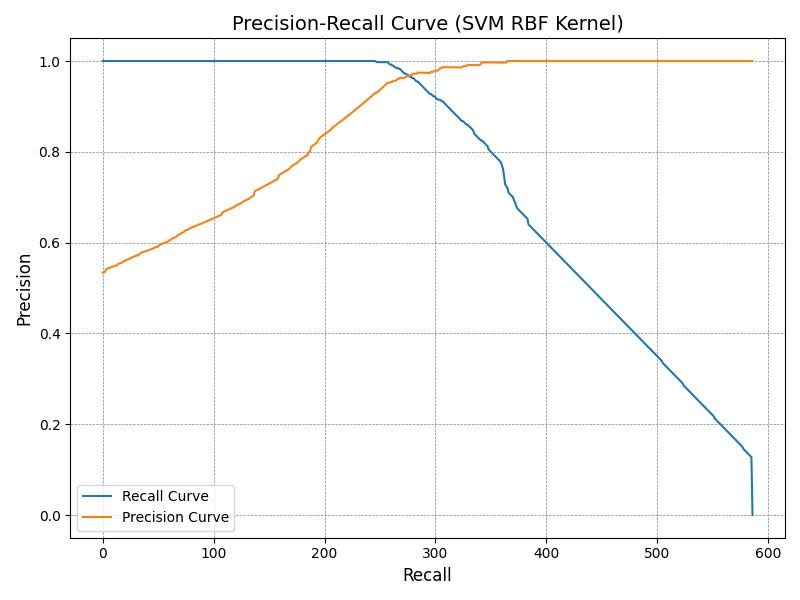
\includegraphics[width=0.95\linewidth]{figures/pre_re_svm.jpeg}
        \captionof{figure}{Precision and Recall: SVM}
        \label{fig:pre-re-svm}
    \end{minipage}
    \vspace{1em}
    \begin{minipage}{0.48\textwidth}
        \centering
        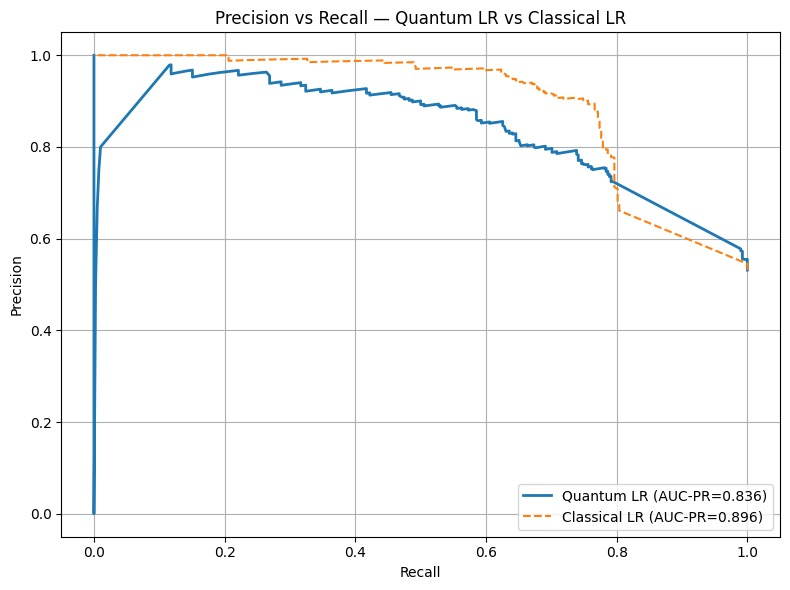
\includegraphics[width=0.95\linewidth]{figures/pr_re_vcq.jpg}
        \captionof{figure}{Precision and Recall Variational Quantum Classifier (VQC)}
        \label{fig:pre-re-rf-qml}
    \end{minipage}
    \hfill
    \begin{minipage}{0.48\textwidth}
        \centering
        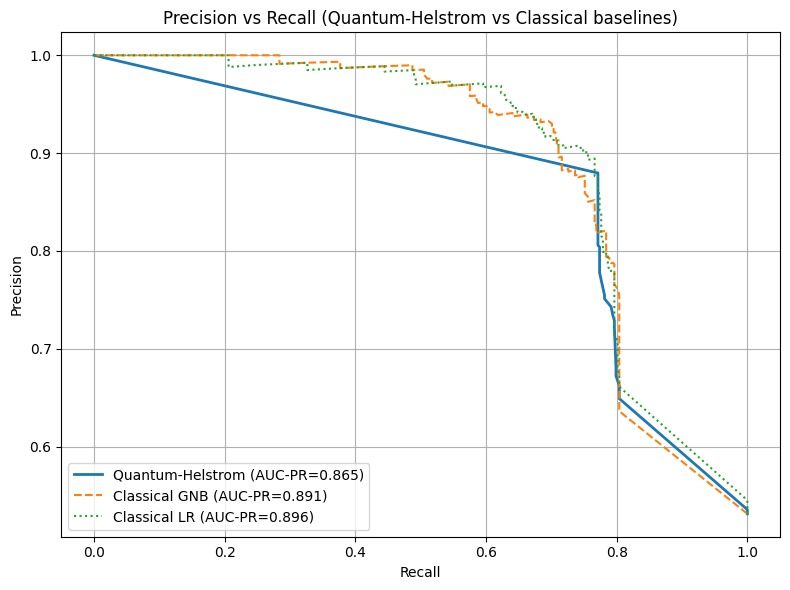
\includegraphics[width=0.95\linewidth]{figures/pr_re_qsvm.jpg}
        \captionof{figure}{Precision and Recall Quantum Kernel}
        \label{fig:pre-re-svm-qml}
    \end{minipage}
\end{figure}

Precision and recall curves for the classical Random Forest (\hyperref[fig:pre-re-rf]{Fig.~\ref{fig:pre-re-rf}}) and Support Vector Machine (\hyperref[fig:pre-re-svm]{Fig.~\ref{fig:pre-re-svm}}) are shown alongside their quantum counterparts: the Variational Quantum Classifier (\hyperref[fig:pre-re-rf-qml]{Fig.~\ref{fig:pre-re-rf-qml}}) and the Quantum Support Vector Machine (\hyperref[fig:pre-re-svm-qml]{Fig.~\ref{fig:pre-re-svm-qml}}).


\subsection{Accuracy and F1 Score of Classical Models}\label{sec:f1score}


\begin{minipage}{0.49\textwidth}
    \centering
    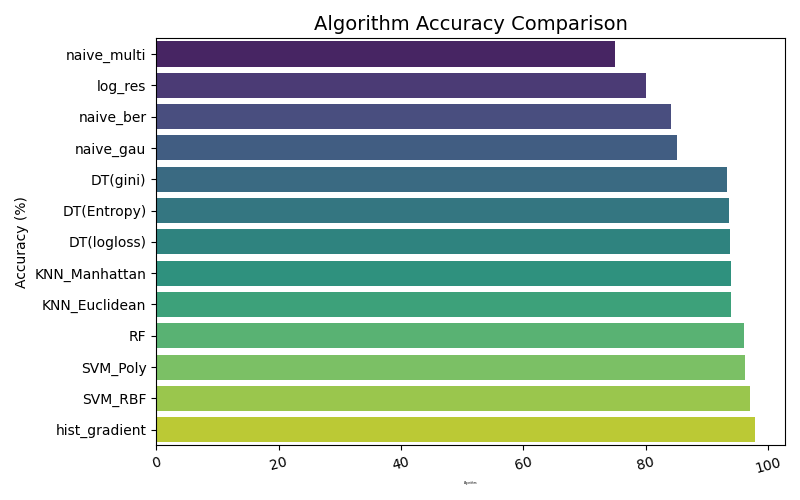
\includegraphics[width=1\linewidth]{figures/accuracy.png}
    \captionof{figure}{\centering Accuracy of the different classification techniques}
    \label{fig:acc}
\end{minipage}
\hfill
\begin{minipage}{0.49\textwidth}
  \centering
    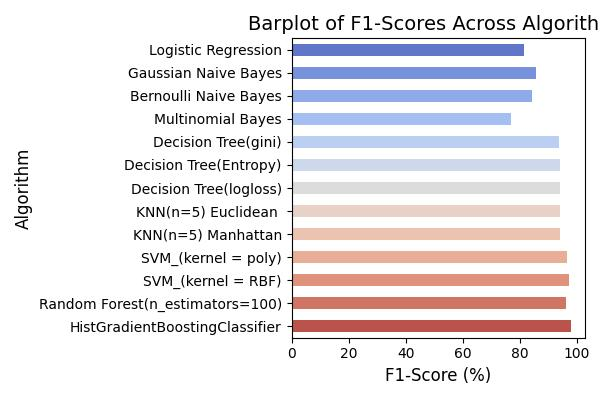
\includegraphics[width=1\linewidth]{figures/f1_score.jpeg}
    \captionof{figure}{\centering F1-score of all the classification models}
    \label{fig:f1_score}
\end{minipage}

\begin{table}[!ht]
    \centering
    \caption{Performance Matrix Including Classical, PCA-Reduced, and Quantum ML Models}
    \renewcommand{\arraystretch}{1.2}
    \setlength{\tabcolsep}{4pt}
    \begin{tabular}{|c|l|c|c|c|c|}
        \hline
        \textbf{No.} & \textbf{Algorithms} & \textbf{Accuracy(\%)} & \textbf{Precision(\%)} & \textbf{Recall(\%)} & \textbf{F1-Score(\%)} \\
        \hline
          1  & Logistic Regression (Full) & 80.11 & 83.38 & 79.51 & 81.40 \\
          \hline
          2 & Naive Bayes (Full) & 85.18 & 88.53 & 83.00 & 85.68 \\
          \hline
          3 & Decision Tree (Full) & 93.72 & 93.53 & 95.12 & 94.32 \\
          \hline
          4 & k-Nearest Neighbor (Full) & 93.99 & 95.17 & 94.30 & 94.33 \\
          \hline
          5 & Support Vector Machine (Full) & 97.06 & 96.32 & 98.25 & 97.28 \\
          \hline
          6 & Random Forest (Full) & 95.99 & 96.95 & 95.50 & 96.22 \\
          \hline
          7 & HGBC (Full) & \textbf{97.86} & \textbf{98.48} & \textbf{97.50} & \textbf{97.90} \\
          \hline
          8 & Logistic Regression (PCA) & 81.71 & 86.15 & 78.14 & 81.95 \\
          \hline
          9 & Naive Bayes (PCA) & 81.97 & 86.83 & 77.89 & 82.12 \\
          \hline
          10 & Decision Tree (PCA) & 95.73 & 96.68 & 95.23 & 95.95 \\
          \hline
          11 & KNN (PCA) & 95.33 & 94.81 & 96.48 & 95.64 \\
          \hline
          12 & SVM (RBF) (PCA) & 88.38 & 95.60 & 81.91 & 88.23 \\
          \hline
          13 & Random Forest (PCA) & 95.59 & 96.20 & 95.48 & 95.84 \\
          \hline
          14 & HGBC (PCA) & 95.86 & 95.53 & 96.73 & 96.13 \\
          \hline
          15 & VQC & 54.87 & 62.00 & 38.94 & 47.84 \\
          \hline
          16 & QSVM & 77.30 & 75.79 & 84.17 & 79.76 \\
          \hline
          17 & QNB & 63.28 & 64.96 & 67.09 & 66.01 \\
          \hline
    \end{tabular}
    \label{tab:Performance_Matrix_Combined}
\end{table}

The performance results based on accuracy, precision, recall, and F1-score are presented in \hyperref[tab:Performance_Matrix_Combined]{Table~\ref{tab:Performance_Matrix_Combined}}. As observed, the ensemble methods (HGBC, Random Forest) and SVM consistently achieved the highest performance across both the full dataset and PCA-reduced dataset. The accuracy of different classification techniques has been presented in a visual representation in \hyperref[fig:acc]{Fig.~\ref{fig:acc}} followed by the F1- Score of the classical classification models in \hyperref[fig:f1_score]{Fig.~\ref{fig:f1_score}}.

Quantum ML models (VQC, QSVM, QNB) performed with accuracies ranging from 55--77\% and moderate F1 scores compared to classical methods. This indicates that, for this dataset, quantum models underperformed relative to classical ensemble methods, consistent with current limitations of near-term quantum circuits on moderately sized datasets.

Quantum models may perform better on tasks with higher-dimensional, strongly non-linear feature spaces where classical kernels struggle, and future work could explore deeper circuits, more expressive encodings, and hybrid quantum-classical architectures to close this gap. Overall, classical ensemble methods remain the most robust approaches for structured tabular classification under current quantum hardware constraints.


\subsection{Comparison Study}\label{sec:results}
\begin{table}[ht!]
    \centering
    \caption{Comparison with Previous ASD Prediction Models (Classical + Quantum)}
    \renewcommand{\arraystretch}{1.3}
    \setlength{\tabcolsep}{6pt}
    \begin{tabular}{|p{5.5cm}|p{2.5cm}|c|c|c|c|}
        \hline
            \textbf{Study} & \textbf{Algorithm} & \textbf{Acc.} & \textbf{Prec.} & \textbf{Rec.} & \textbf{F1} \\
            \hline
            Lee et al.\ \cite{lee2020}
            & Naive Bayes     & 73    & --    & --    & 78   \\
            & CVM              & 87    & --    & --    & 83.6 \\
            & Random Forest    & 87.1  & --    & --    & 86.8 \\
            \hline
            Rasul et al.\ \cite{rasul2024}
            & Random Forest    & 94    & 90.1  & 88.3  & --   \\
            & Naive Bayes      & 85    & 84    & 81    & --   \\
            & SVM              & 80    & 81    & 80    & --   \\
            \hline
            Akter et al.\ \cite{akter2019}
            & Naive Bayes      & 96    & --    & --    & 97   \\
            & SVM              & 85    & --    & --    & --   \\
            & KNN              & 90    & --    & --    & --   \\
            & Random Forest    & \textbf{99} & -- & -- & --   \\
            \hline
            Farooq et al.\ \cite{farooq2023}
            & Logistic Regression & 97.15 & -- & -- & 98   \\
            & Naive Bayes         & 94    & -- & -- & 96   \\
            & KNN                 & 90.52 & -- & -- & 93   \\
            & Random Forest       & 81.52 & -- & -- & 88   \\
            \hline
            Saranya \& Menaka \cite{saranya2025}
            & QSVM             & 98.9  & --   & --   & --   \\
            \hline
    \end{tabular}
    \label{tab:Comparative_Studies}
\end{table}
Our methods were compared with recent studies in the literature, with a concise summary presented in Table~\ref{tab:Comparative_Studies}. The HGBC model outperformed most reported classical approaches, achieving 97.86\% accuracy and a 97.90\% F1-score. While some quantum-based methods, such as QSVM, report accuracies up to 98.9\%, these results often rely on specialized feature engineering or smaller, carefully curated datasets.

Several prior studies are affected by class imbalance, limited feature diversity, high dimensionality, noise, or overfitting. In contrast, our pipeline employed balanced data, systematic pre-processing, and hyperparameter tuning to improve robustness and generalization.

The higher QSVM accuracy reported in \cite{saranya2025} can be attributed to an enhanced, dataset-specific feature set and a relatively small, well-structured dataset, which improved class separability and kernel effectiveness. Our QML experiments, conducted on PCA-reduced features from a larger and more overlapping dataset, faced greater classification complexity, limiting achievable performance. This suggests that quantum models are most effective in structured, lower-dimensional, and well-separated feature spaces, and may benefit from hybrid classical--quantum pipelines.

Finally, this work does not evaluate real quantum hardware. All QML experiments were performed using PennyLane (VQC, QNB) and Qiskit Aer (QSVM) quantum simulators, providing a realistic benchmark under near-term hardware constraints rather than demonstrating performance on physical quantum devices.


\section{Conclusion}
\label{sec:conclusion}

This study systematically compared classical supervised machine learning models with Quantum Machine Learning (QML) approaches for ASD trait prediction on non-linear datasets. Among classical methods, the Histogram Gradient Boosting Classifier (HGBC) achieved the strongest overall performance, reaching 97.86\% accuracy and consistently outperforming other baselines.

Within the quantum models, QSVM achieved the highest quantum accuracy at 77.30\%, followed by QNB at 63.28\% and VQC at 54.87\%. The VQC's near-random performance despite 50 training epochs reflects the barren plateau problem: with only 12~trainable parameters in a single variational layer, the loss landscape becomes flat and the optimiser fails to converge. QNB and QSVM, which use no trainable quantum parameters and instead rely on fixed feature maps (data re-uploading and ZZFeatureMap respectively), avoid this optimisation difficulty but still lack the expressivity to match classical ensemble methods on this dataset. These results indicate that current near-term quantum circuits with shallow depth and limited qubits are insufficient to compete with well-tuned classical models on structured tabular data.

Exploratory Data Analysis further revealed higher ASD trait prevalence in children (60.57\%) and males, along with demographic patterns related to ethnicity and family history, highlighting the multifactorial nature of ASD.

Overall, classical ensemble models such as HGBC and Random Forest remain the most reliable under current computational constraints. However, quantum-based approaches present a promising direction, particularly without dimensionality reduction. Future work will focus on larger datasets, richer clinical feature sets, hybrid classical--quantum architectures, and further hyperparameter optimization of kernel-based quantum models to better compete with state-of-the-art classical methods.




\begin{thebibliography}{13}

\bibitem{vakadkar2021}
Vakadkar, K., Purkayastha, D. and Krishnan, D. (2021) Detection of Autism Spectrum Disorder in Children Using Machine Learning Techniques. \emph{SN Computer Science} \textbf{2}, 386.

\bibitem{saranya2025}
Saranya, S. and Menaka, R. (2025) A Quantum-Based Machine Learning Approach for Autism Detection using Common Spatial Patterns of EEG Signals. \emph{IEEE Access} \textbf{13}, 15739--15750.

\bibitem{lee2020}
Lee, Scott H. and Maenner, Matthew J. and Heilig, Charles M. (2020) A Comparison of Machine Learning Algorithms for the Surveillance of Autism Spectrum Disorder. \emph{Proceedings of IJ-CSE}, Atlantis Press.



\bibitem{nogay2020}
Nogay, H. S. and Adeli, H. (2020) Machine learning (ML) for the diagnosis of autism spectrum disorder (ASD) using brain imaging. \emph{Reviews in the Neurosciences} \textbf{31}(8), 825--841.


\bibitem{kotsiantis2006}
Kotsiantis, S., Kanellopoulos, D. and Pintelas, P. (2006) Data Preprocessing for Supervised Learning. \emph{International Journal of Computer Science} \textbf{1}, 111--117.

\bibitem{hosmer2000}
Hosmer, D. W. and Lemeshow, S. (2000) \emph{Applied Logistic Regression}. 2nd edition. Wiley, New York.

\bibitem{breiman2001}
Breiman, L. (2001) Random Forests. \emph{Machine Learning} \textbf{45}(1), 5--32.


\bibitem{hearst1998}
Hearst, M. A., Dumais, S. T., Osuna, E., Platt, J. and Scholkopf, B. (1998) Support vector machines. \emph{IEEE Intelligent Systems and their Applications} \textbf{13}(4), 18--28.

\bibitem{schuld2020}
Schuld, M., Bocharov, A., Svore, K. M., \& Wiebe, N. (2020). Circuit-centric quantum classifiers. \emph{Physical Review A}, 101(3), 032308.

\bibitem{havlivcek2019}
Havl\'{i}\v{c}ek, V., C\'{o}rcoles, A. D., Temme, K., Harrow, A. W., Kandala, A., Chow, J. M., \& Gambetta, J. M. (2019). Supervised learning with quantum-enhanced feature spaces. \emph{Nature}, 567(7747), 209--212.


\bibitem{bishop2006}
Bishop, C. M. (2006) \emph{Pattern Recognition and Machine Learning}. Springer, New York, NY.

\bibitem{rasul2024}
Rasul, R. A., Saha, P., Bala, D., Karim, S. R., Abdullah, M. I. and Saha, B. (2024) An evaluation of machine learning approaches for early diagnosis of autism spectrum disorder. \emph{Healthcare Analytics} \textbf{5}, 100293.

\bibitem{akter2019}
Akter, T., Shahriare Satu, M., Khan, M. I., Ali, M. H., Uddin, S., Lio, P., Quinn, J. M. W. and Moni, M. A. (2019) Machine learning-based models for early stage detection of autism spectrum disorders. \emph{IEEE Access} \textbf{7}, 166509--166527.

\bibitem{farooq2023}
Farooq, M. S., Tehseen, R., Sabir, M. and Atal, Z. (2023) Detection of autism spectrum disorder (ASD) in children and adults using machine learning. \emph{Scientific Reports} \textbf{13}, 9605.

\bibitem{asddataset}
CircuitOvertime (2023) ASD Binary Classification Dataset. Kaggle. Available at: \url{https://www.kaggle.com/datasets/circuitovertime/asd-binary-classification}. Accessed: 2025-04-20.

\bibitem{perez2020}
P\'{e}rez-Salinas, A., Cervera-Lierta, A., Gil-Fuster, E. and Latorre, J. I. (2020) Data re-uploading for a universal quantum classifier. \emph{Quantum} \textbf{4}, 226.

\end{thebibliography}
\end{document}